Se ha creado la interfaz en base a los bocetos de la sección anterior.
La interfaz se ha desarrollado en React.

\subsubsection{Descripción de los recursos empleados en la interfaz}
La primera tarea que se ha realizado ha sido la de definir los colores y tipografías que se van a utilizar en la interfaz.
Se ha elegido la tipografía \textit{Pokemon Hollow} para el título de la aplicación y para la bienvenida al usuario.

El logo de la aplicación se ha generado mediante inteligencia artificial, utilizando la herramienta \coloredUnderline{\href{https://openai.com/chatgpt/}{ChatGPT}}.
, al igual que el \textit{favicon} de la aplicación.

Los avatares que se pueden seleccionar como imagen de perfil se han obtenido de la página web \coloredUnderline{\href{https://www.behance.net/gallery/10774061/Pokmon-Avatars}{Behance, Pokémon Avatars de Mikeel Araña}}.

Las imágenes de las medallas de los gimnasios se han obtenido de la página web \coloredUnderline{\href{https://www.wikidex.net/wiki/Líder_de_gimnasio}{Wikidex}}.

Los iconos de los tipos de Pokémon se han obtenido del repositorio \coloredUnderline{\href{https://github.com/duiker101/pokemon-type-svg-icons}{pokemon-type-svg-icons, de duiker101}}.

Las imágenes de los Pokémon se han obtenido de la página web \coloredUnderline{\href{https://pokeapi.co/}{PokéAPI}}.

Para implementar la interfaz se ha utilizado principalmente la biblioteca \coloredUnderline{\href{https://material-ui.com/}{Material-UI}}. 


\subsubsection{Interfaz de la aplicación}
A continuación se muestran las pantallas de las páginas principales de la aplicación.
Pueden diferir ligeramente de los bocetos iniciales, ya que se han realizado ajustes para mejorar la usabilidad y la estética de la aplicación.

\begin{figure}[H]
    \centering
    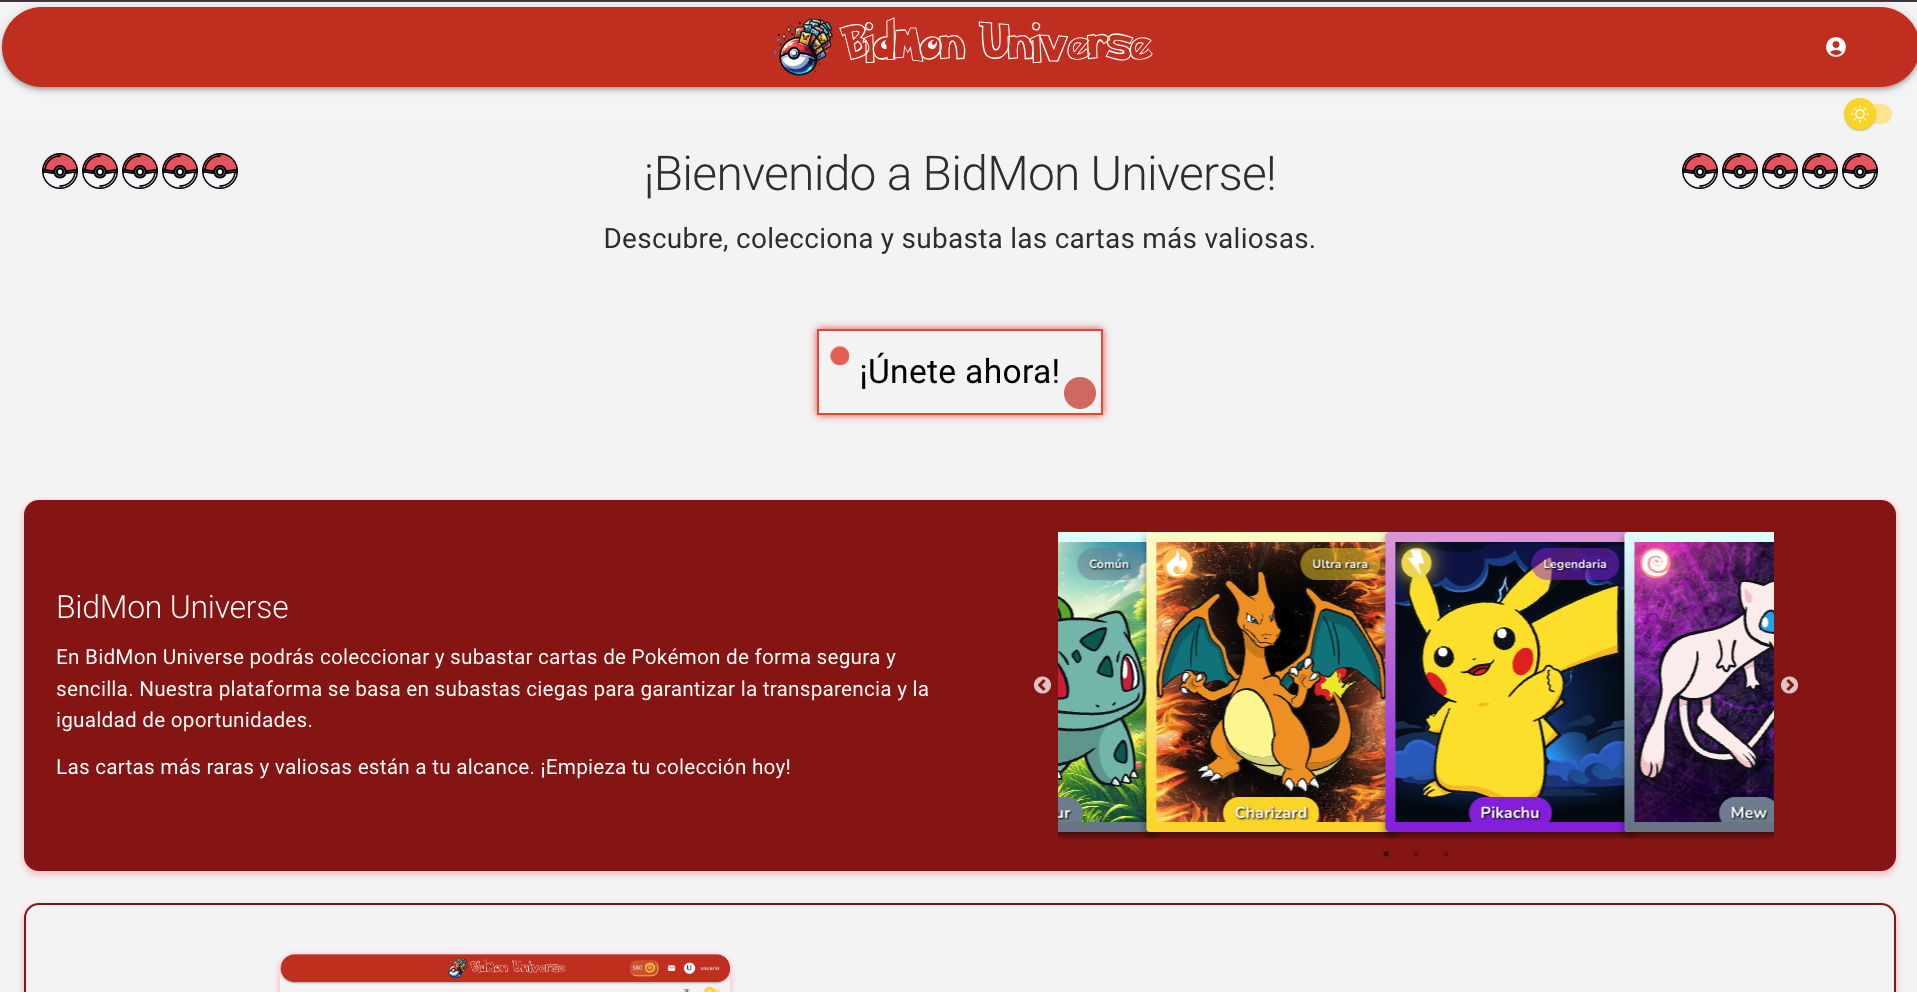
\includegraphics[width=0.8\textwidth]{figures/6-Analisis/6-Interfaz/interfaz/home.png}
    \caption{Página Home, página de inicio de la aplicación.}
    \label{fig:interfaz-home}
\end{figure}

\begin{figure}[H]
    \centering
    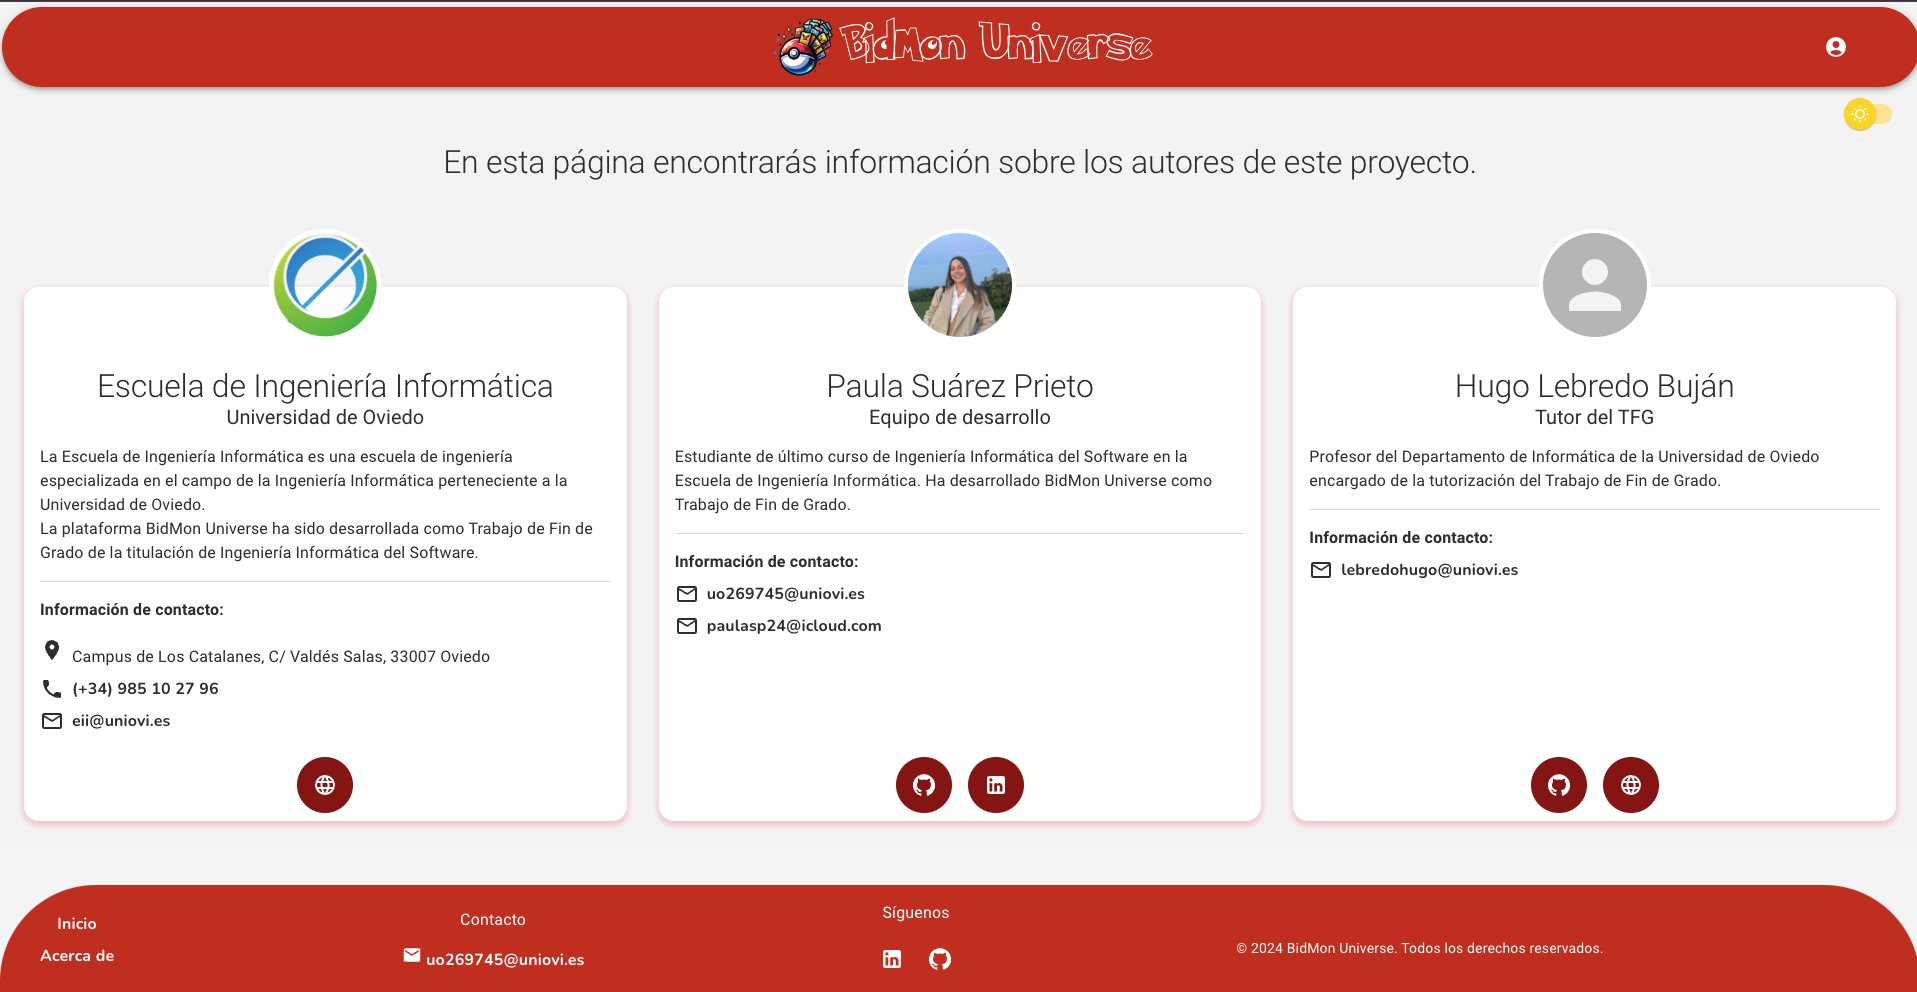
\includegraphics[width=0.8\textwidth]{figures/6-Analisis/6-Interfaz/interfaz/about.png}
    \caption{Página de información sobre la aplicación.}
    \label{fig:interfaz-about}
\end{figure}

\begin{figure}[H]
    \centering
    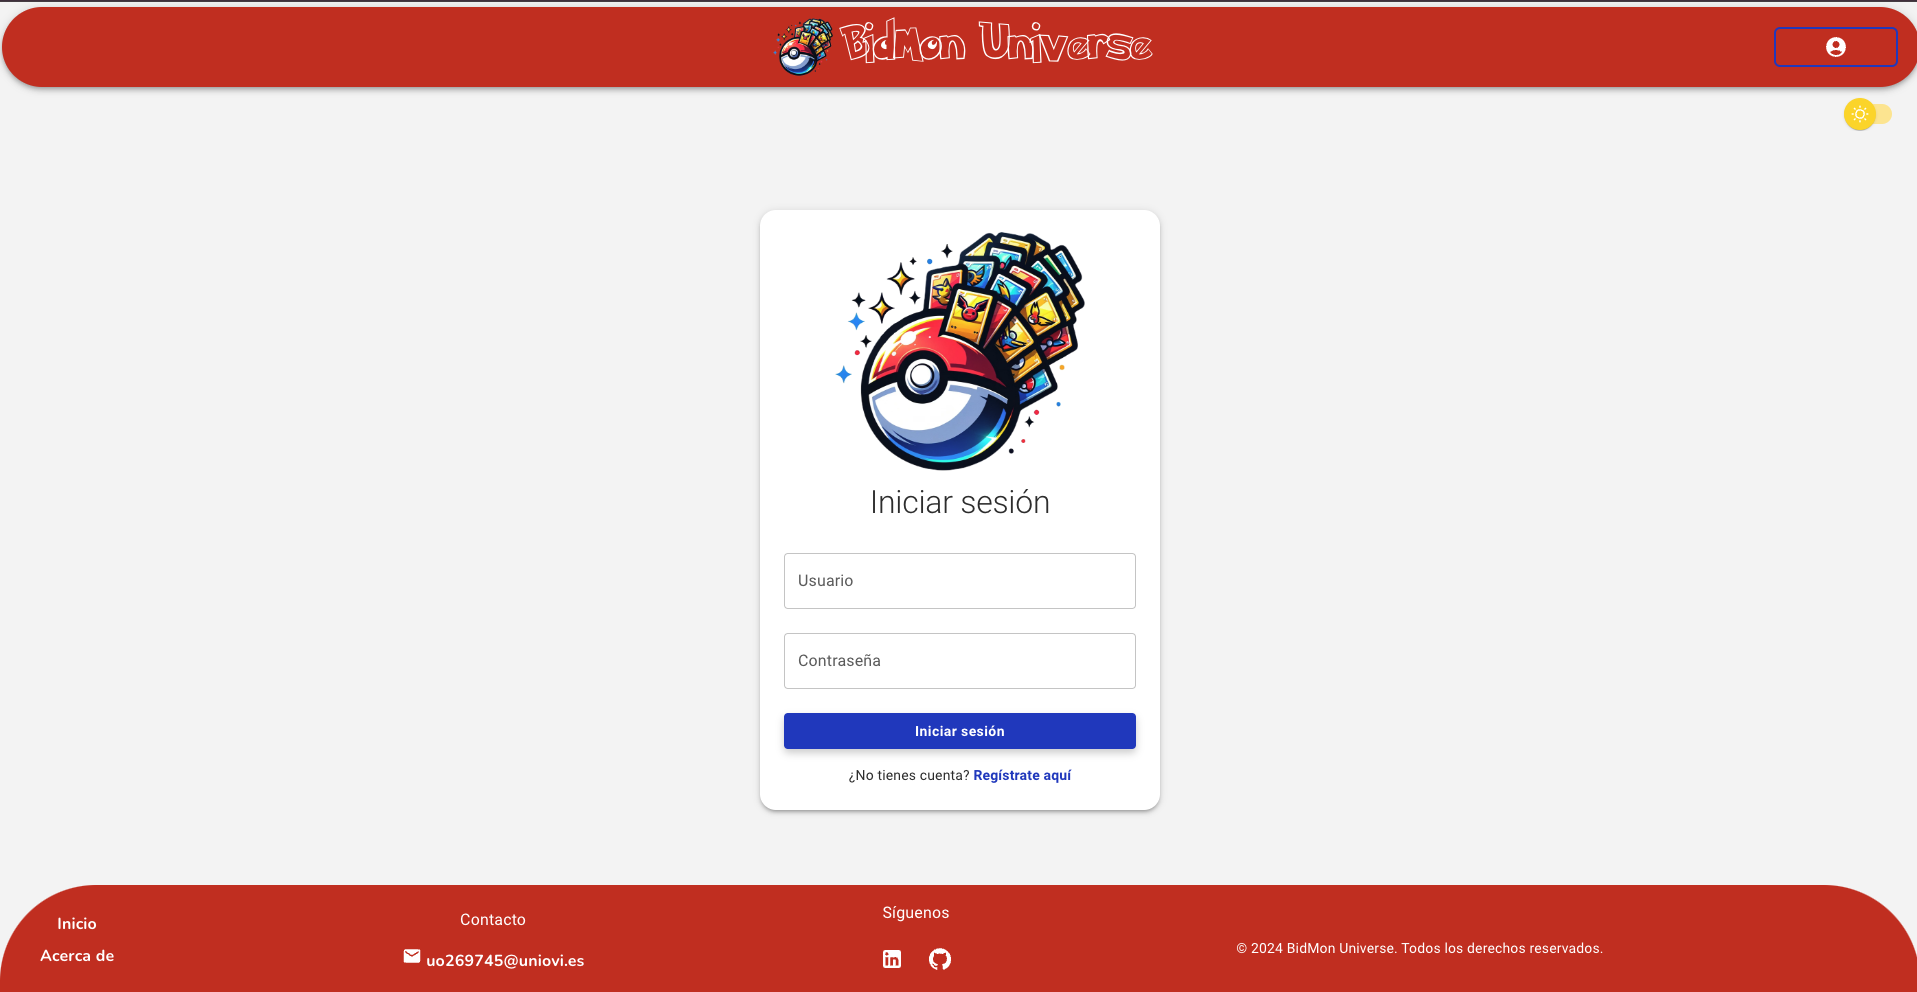
\includegraphics[width=0.8\textwidth]{figures/6-Analisis/6-Interfaz/interfaz/login.png}
    \caption{Página de inicio de sesión.}
    \label{fig:interfaz-login}
\end{figure}

\begin{figure}[H]
    \centering
    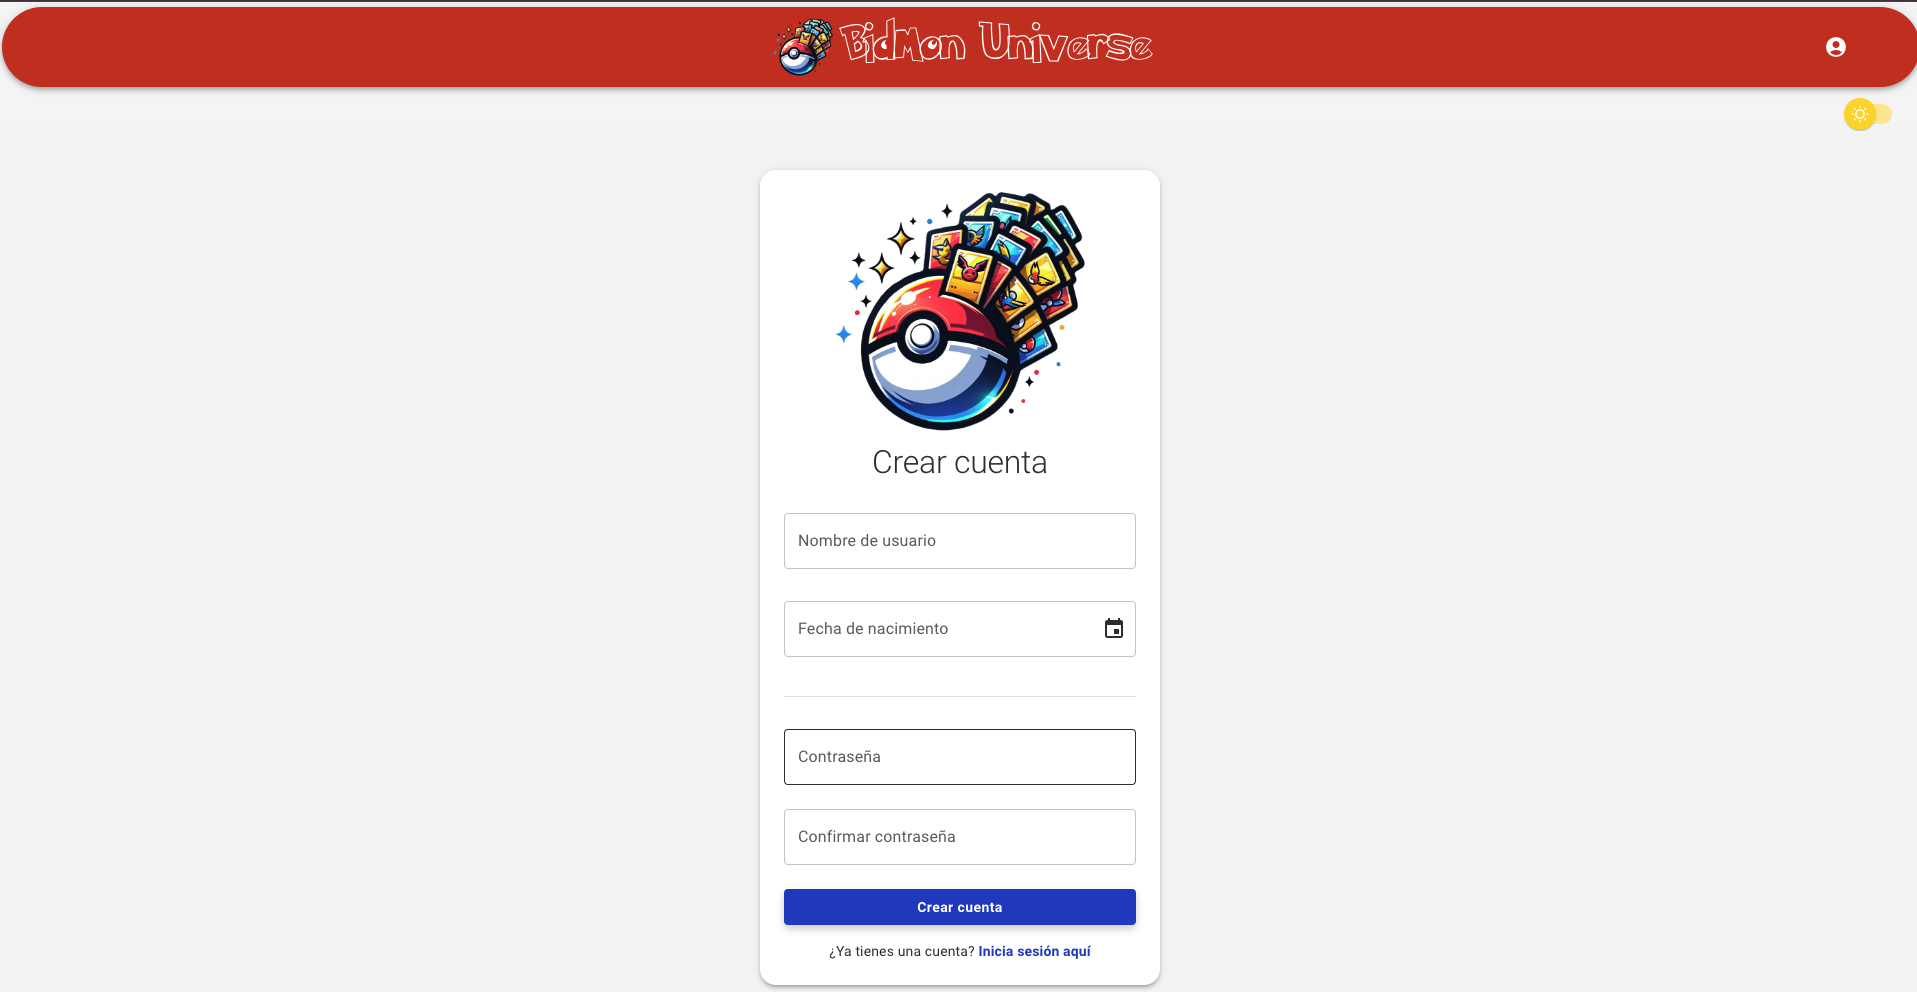
\includegraphics[width=0.8\textwidth]{figures/6-Analisis/6-Interfaz/interfaz/signup.png}
    \caption{Página de registro de usuario.}
    \label{fig:interfaz-registro}
\end{figure}

\begin{figure}[H]
    \centering
    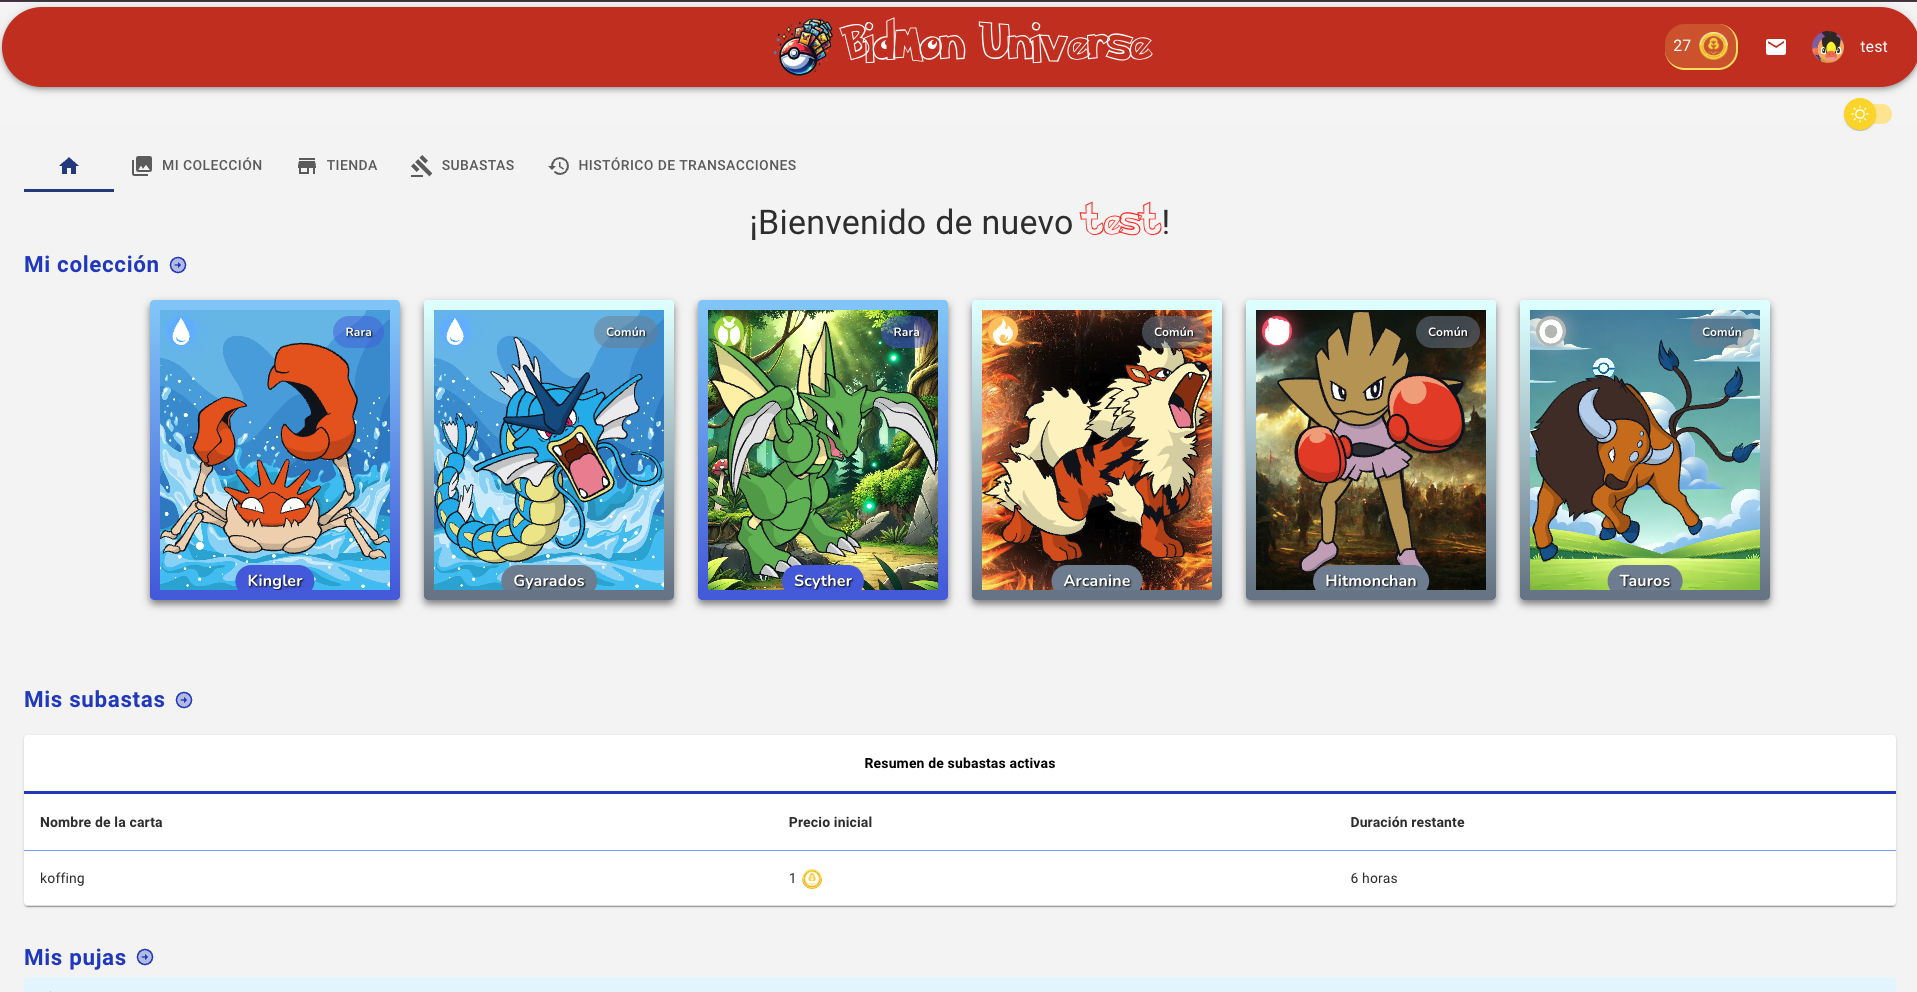
\includegraphics[width=0.8\textwidth]{figures/6-Analisis/6-Interfaz/interfaz/logued.png}
    \caption{Página principal de la aplicación, una vez que el usuario ha iniciado sesión.}
    \label{fig:interfaz-logued}
\end{figure}


\begin{figure}[H]
    \centering
    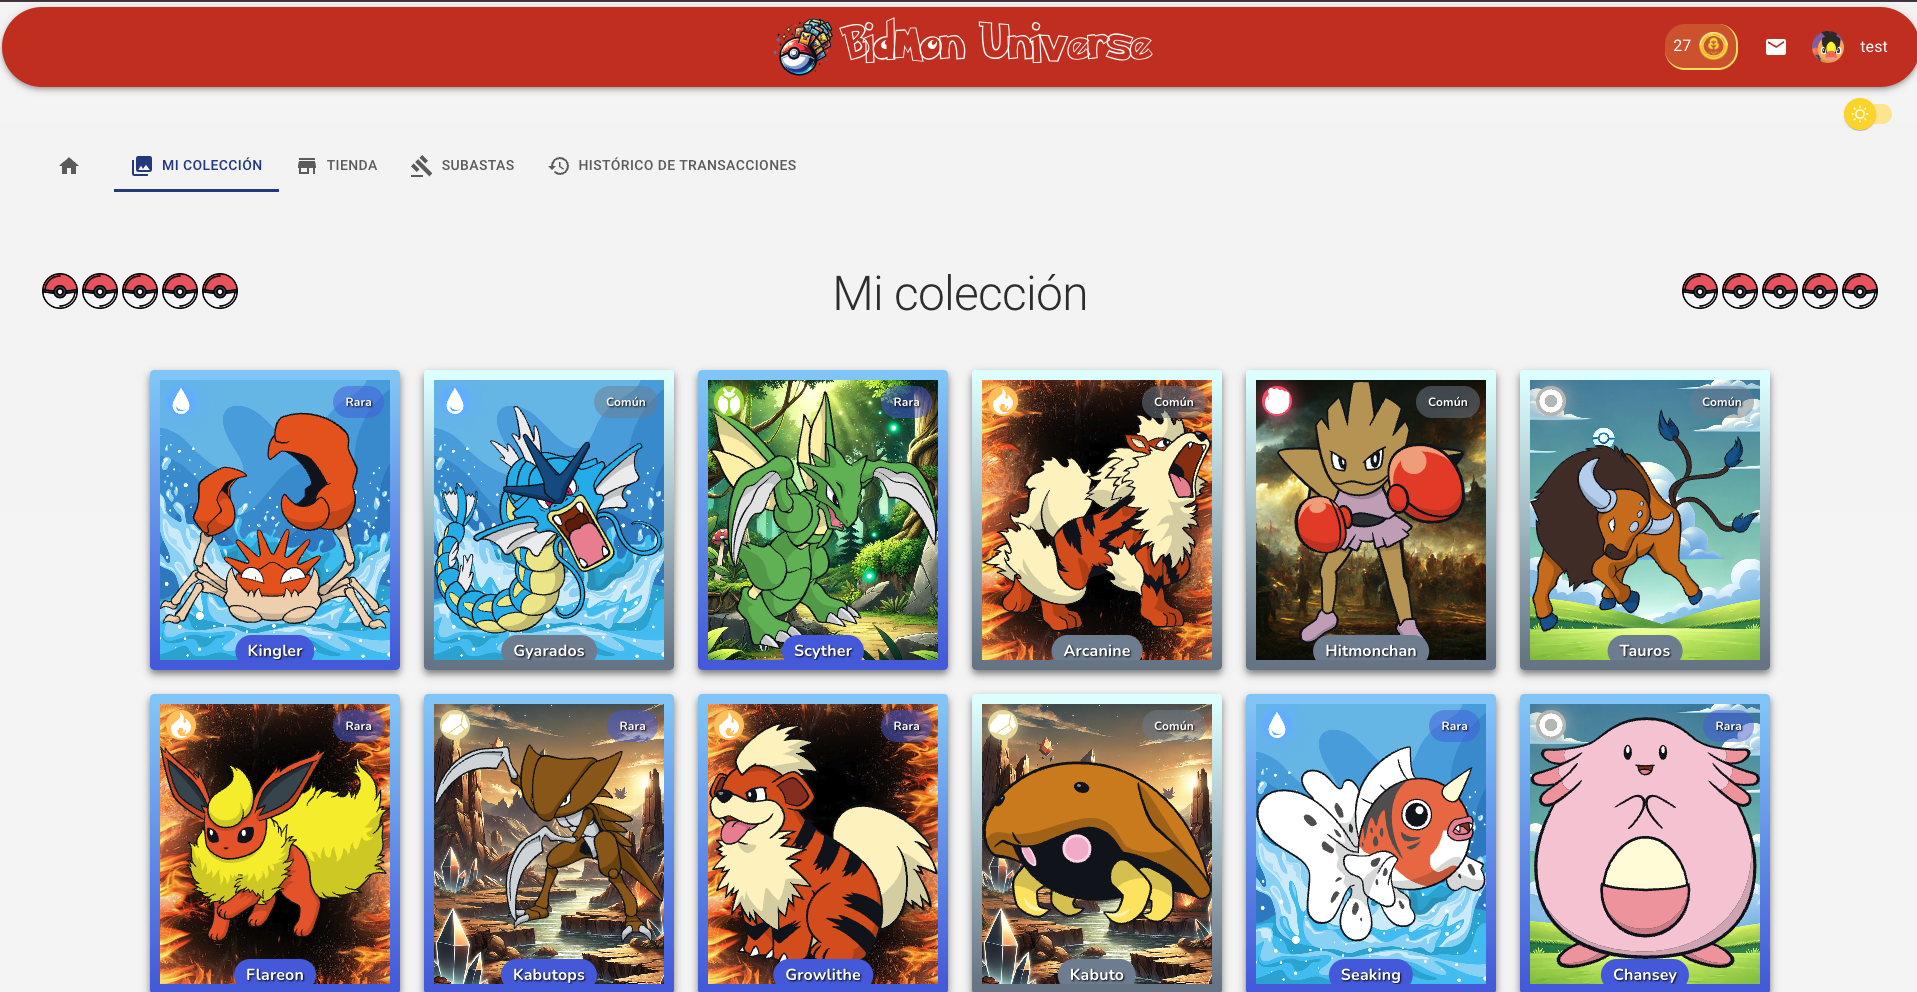
\includegraphics[width=0.8\textwidth]{figures/6-Analisis/6-Interfaz/interfaz/coleccion.png}
    \caption{Página de la colección de cartas del usuario.}
    \label{fig:interfaz-coleccion}
\end{figure}


\begin{figure}[H]
    \centering
    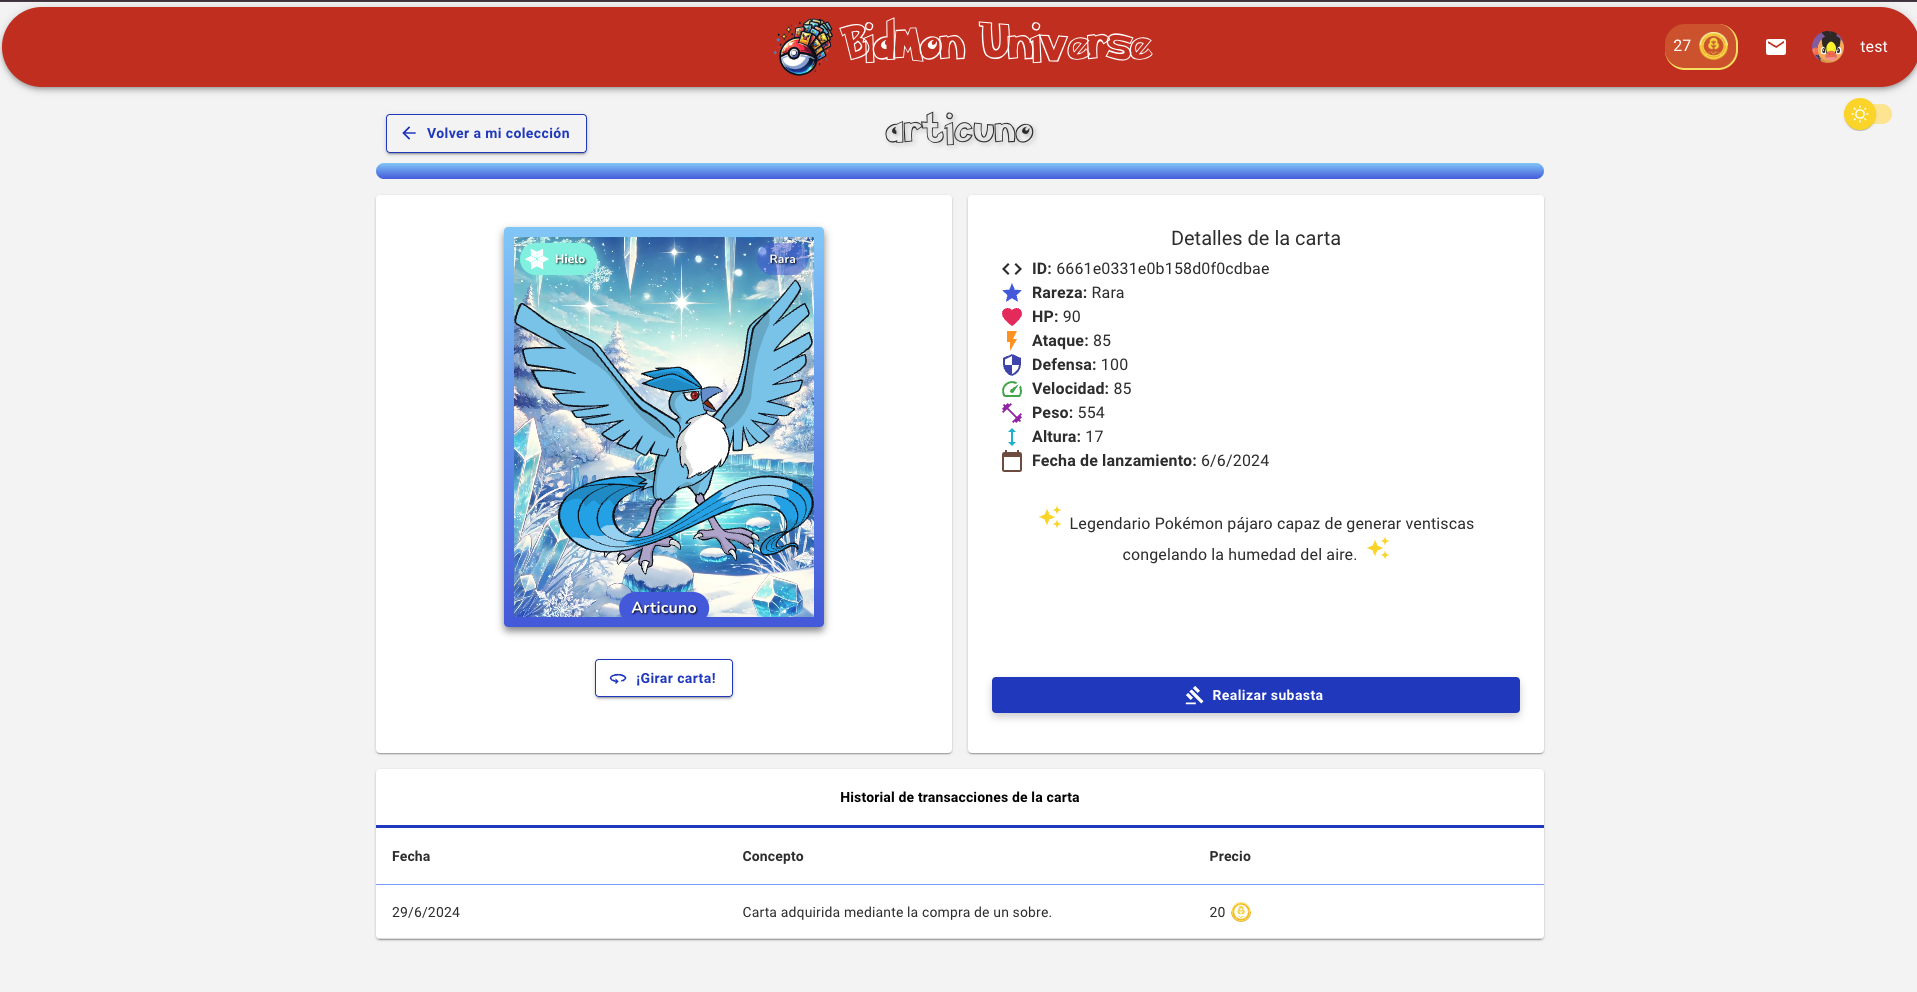
\includegraphics[width=0.8\textwidth]{figures/6-Analisis/6-Interfaz/interfaz/detalle_carta.png}
    \caption{Página de detalle de una carta de la colección del usuario.}
    \label{fig:interfaz-detalle-carta}
\end{figure}


\begin{figure}[H]
    \centering
    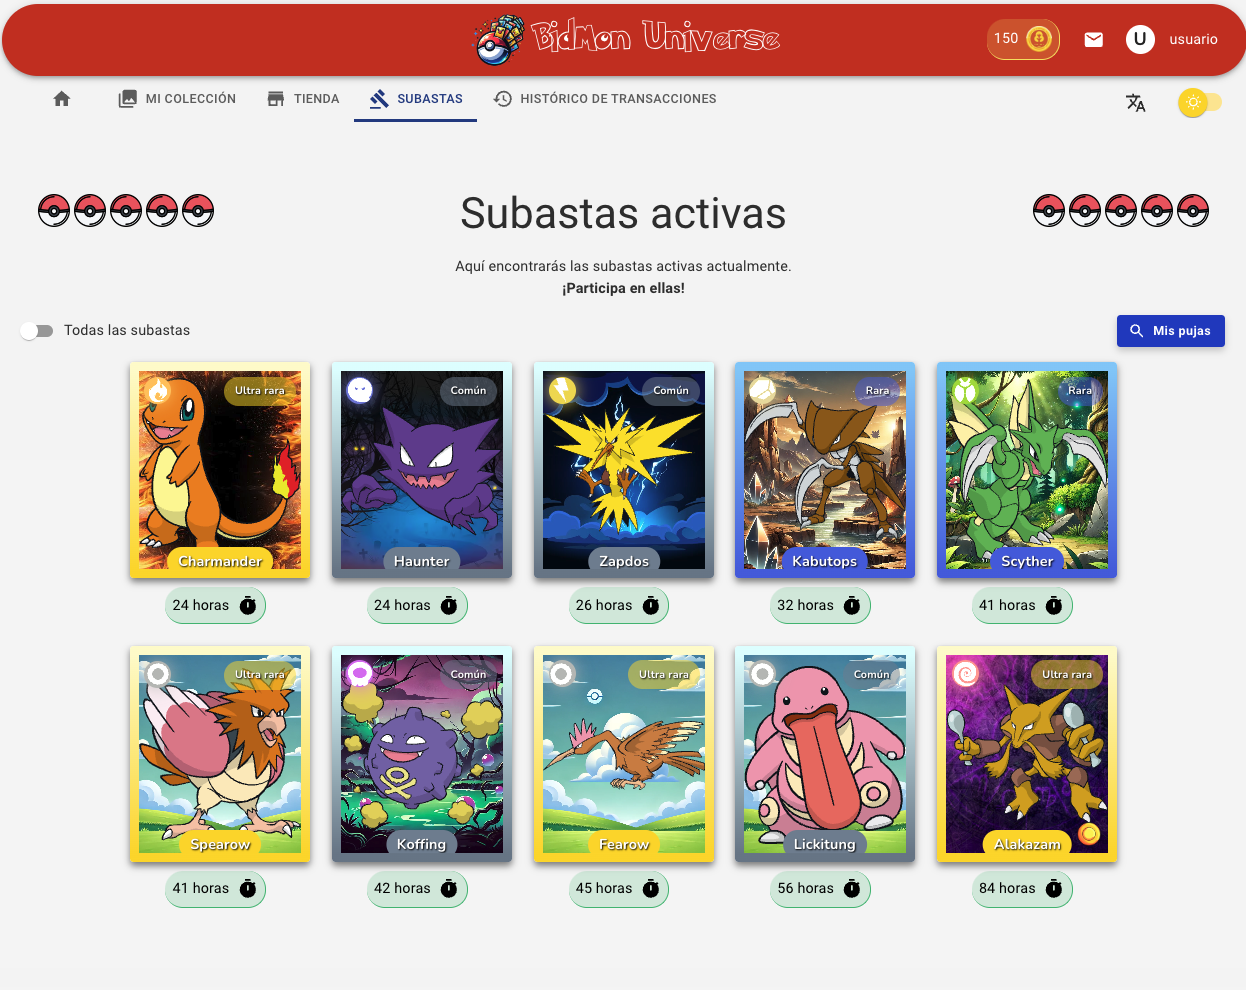
\includegraphics[width=0.8\textwidth]{figures/6-Analisis/6-Interfaz/interfaz/subastas.png}
    \caption{Página de las subastas activas de cartas.}
    \label{fig:interfaz-subastas}
\end{figure}


\begin{figure}[H]
    \centering
    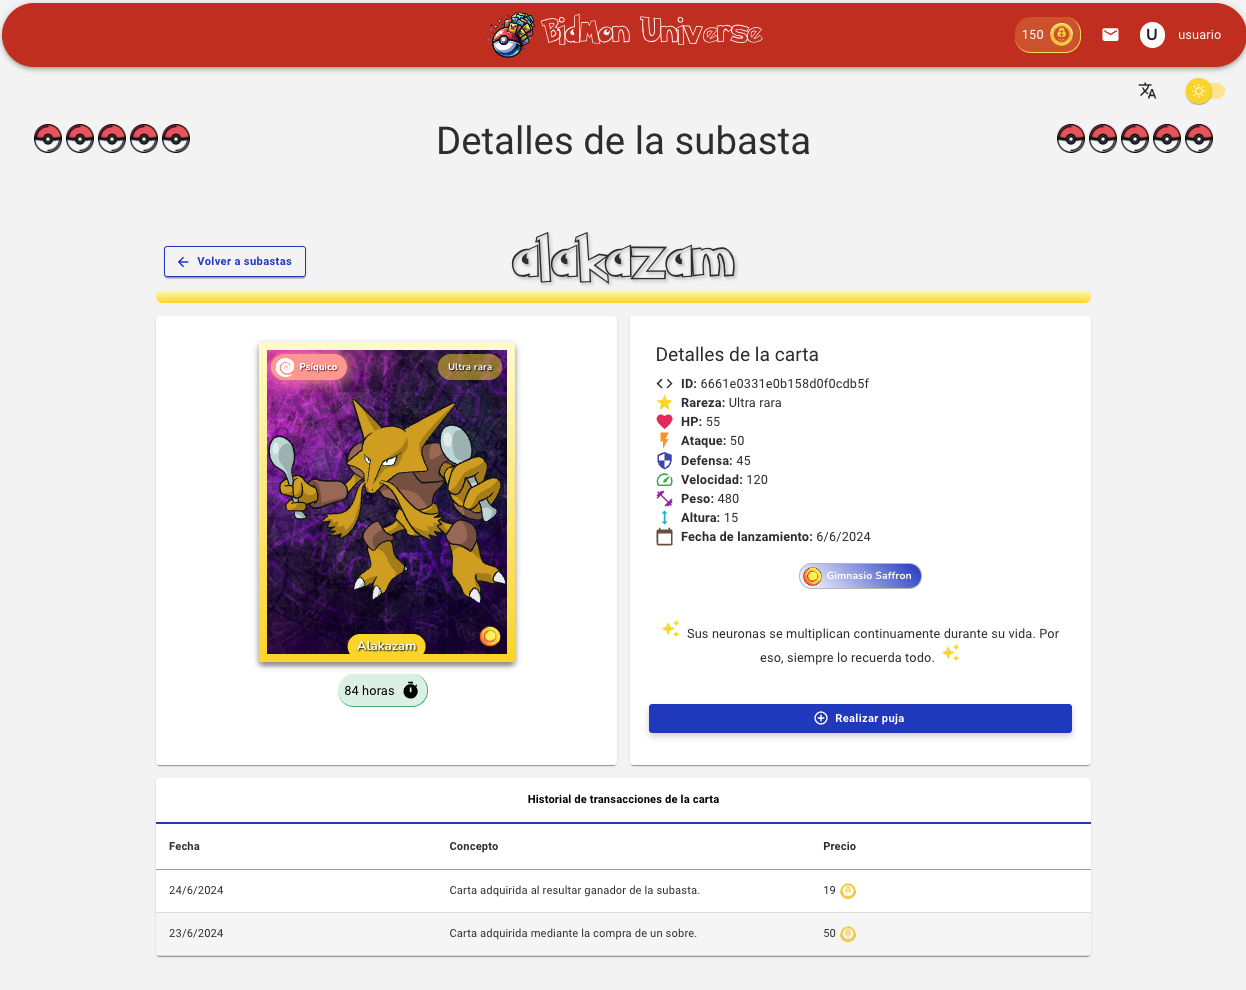
\includegraphics[width=0.8\textwidth]{figures/6-Analisis/6-Interfaz/interfaz/detalle_subasta.png}
    \caption{Página de detalle de una subasta activa.}
    \label{fig:interfaz-detalle-subasta}
\end{figure}

\begin{figure}[H]
    \centering
    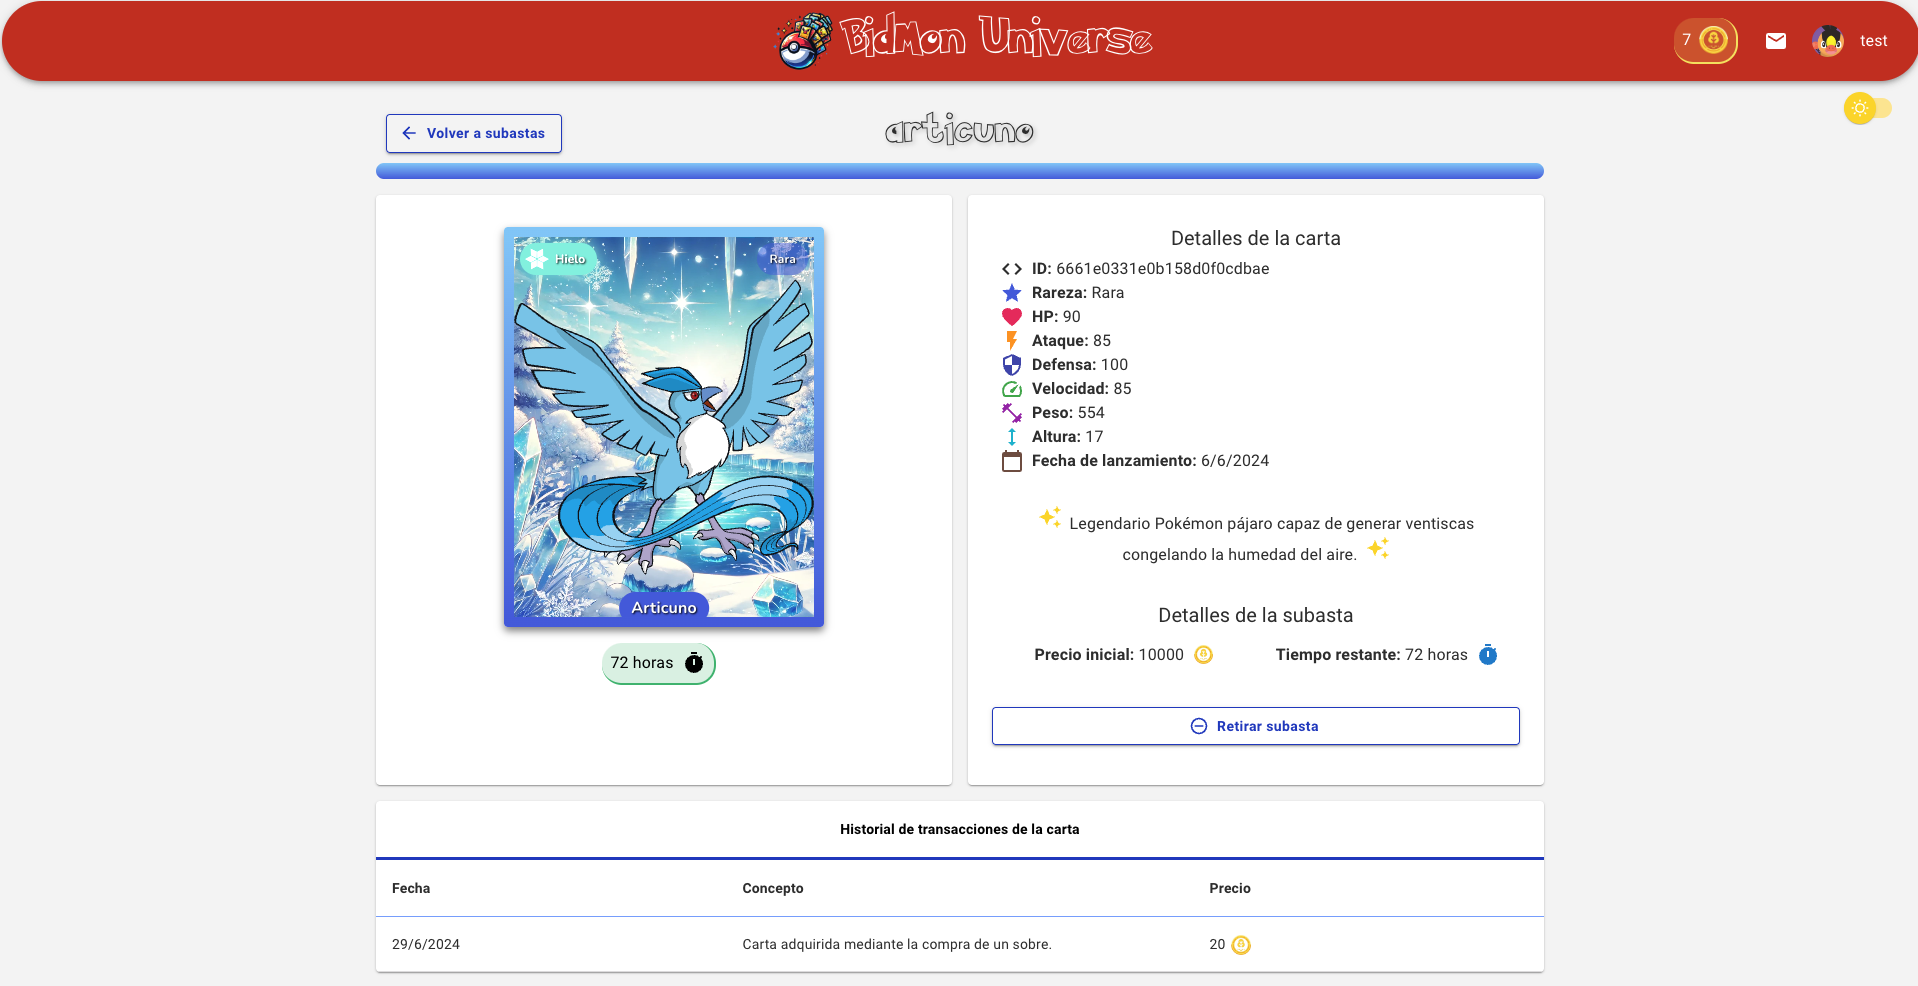
\includegraphics[width=0.8\textwidth]{figures/6-Analisis/6-Interfaz/interfaz/mi_subasta_detalle.png}
    \caption{Página de detalle de una subasta activa creada por el usuario.}
    \label{fig:interfaz-detalle-mi-subasta}
\end{figure}


\begin{figure}[H]
    \centering
    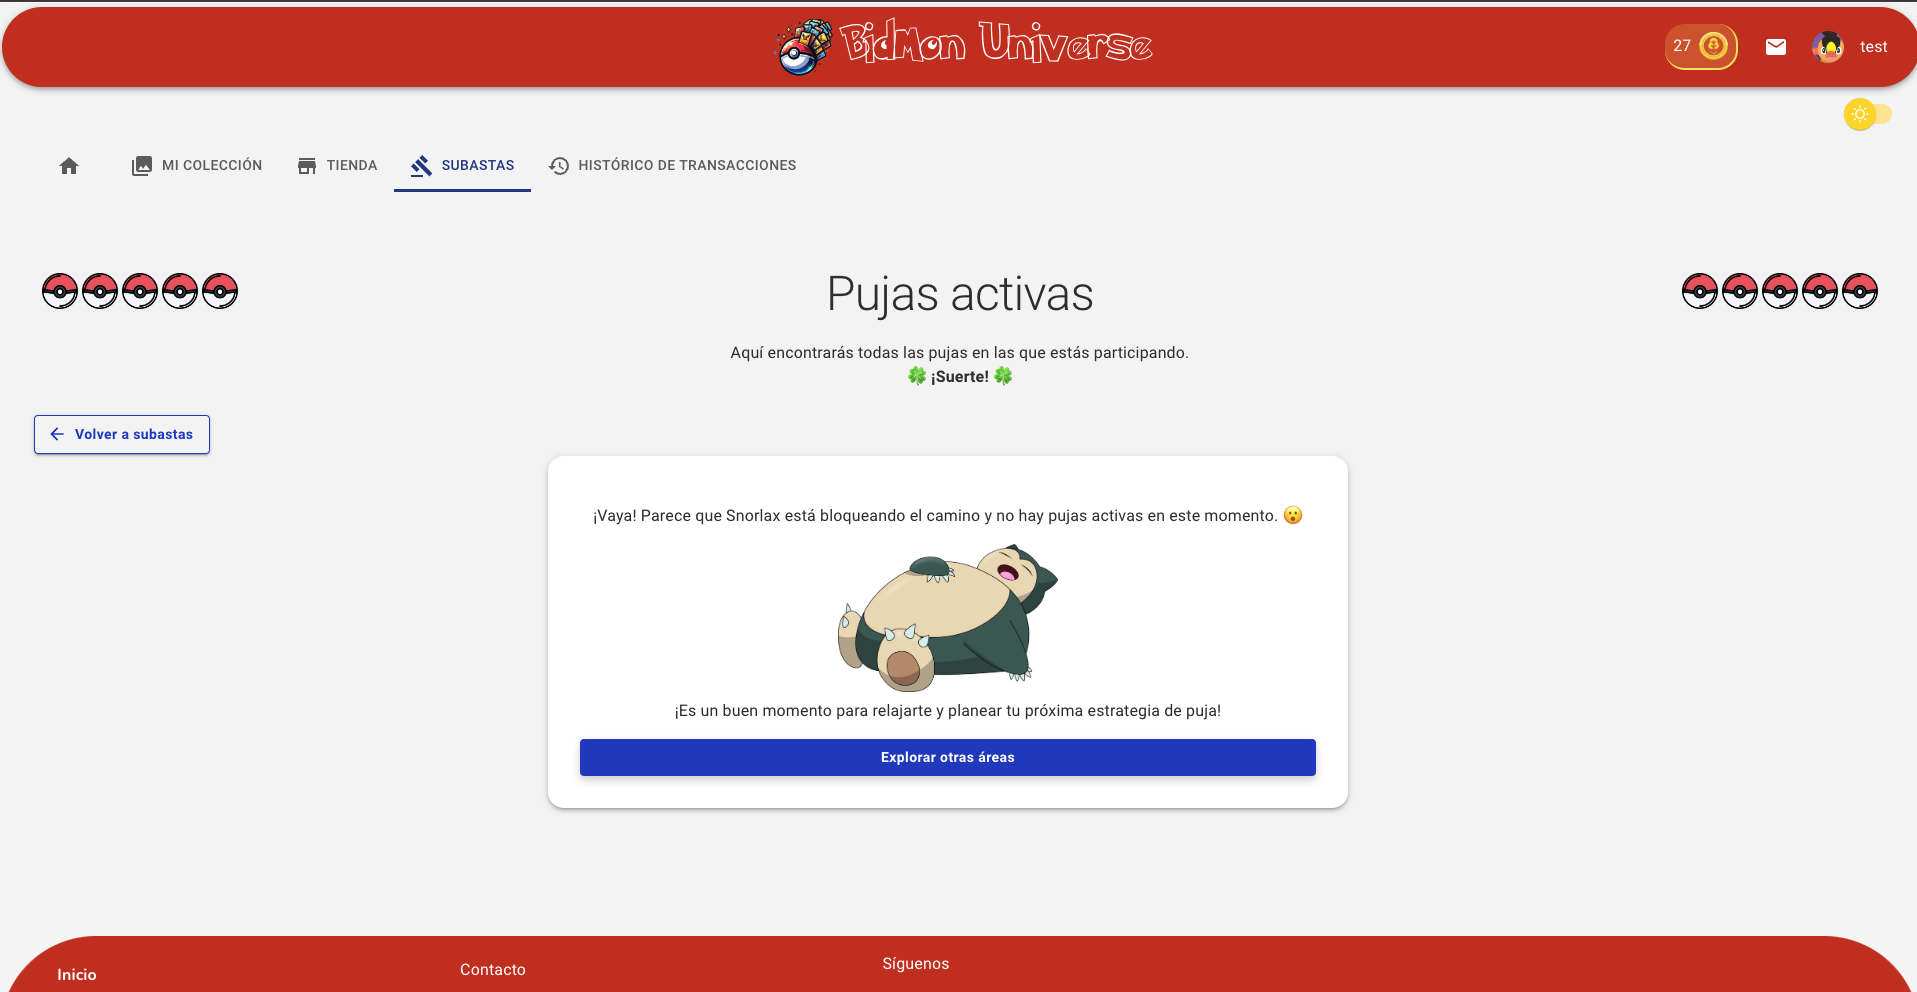
\includegraphics[width=0.8\textwidth]{figures/6-Analisis/6-Interfaz/interfaz/pujas.png}
    \caption{Página de pujas activas del usuario en subastas.}
    \label{fig:interfaz-gimnasios}
\end{figure}


\begin{figure}[H]
    \centering
    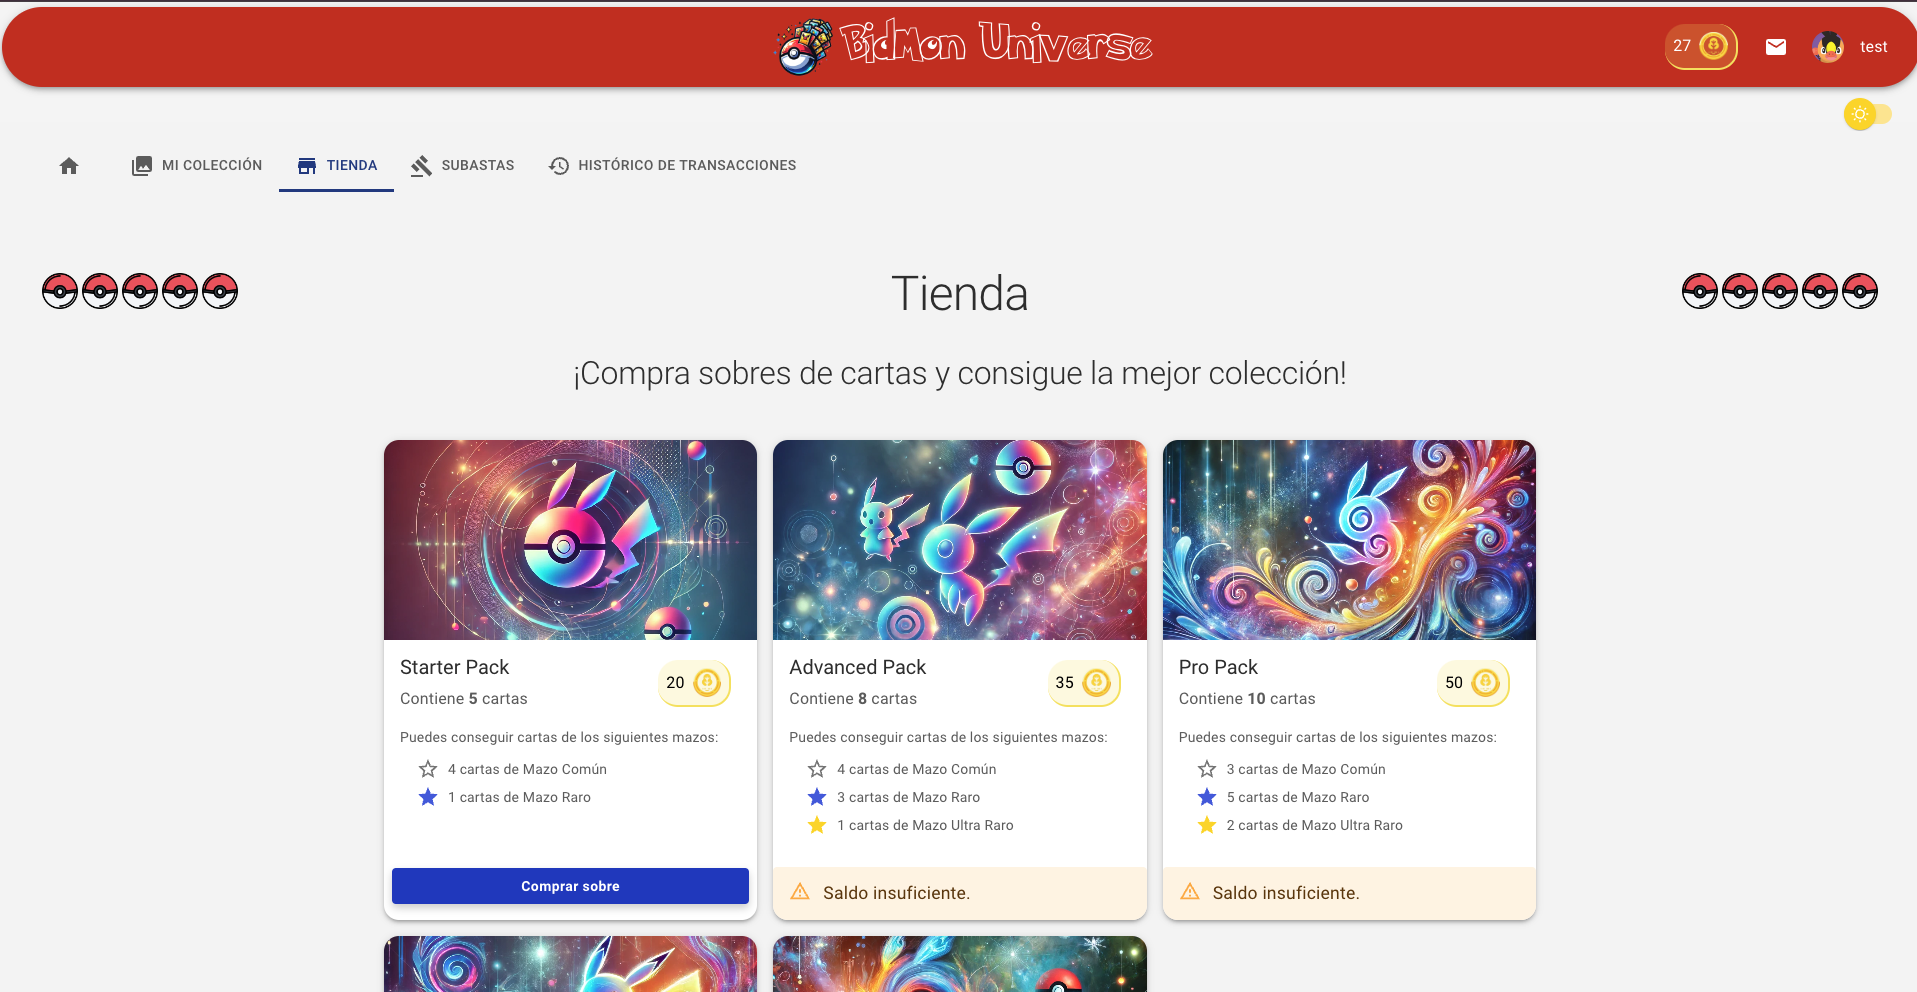
\includegraphics[width=0.8\textwidth]{figures/6-Analisis/6-Interfaz/interfaz/tienda.png}
    \caption{Página de la tienda de sobres de cartas.}
    \label{fig:interfaz-tienda}
\end{figure}


\begin{figure}[H]
    \centering
    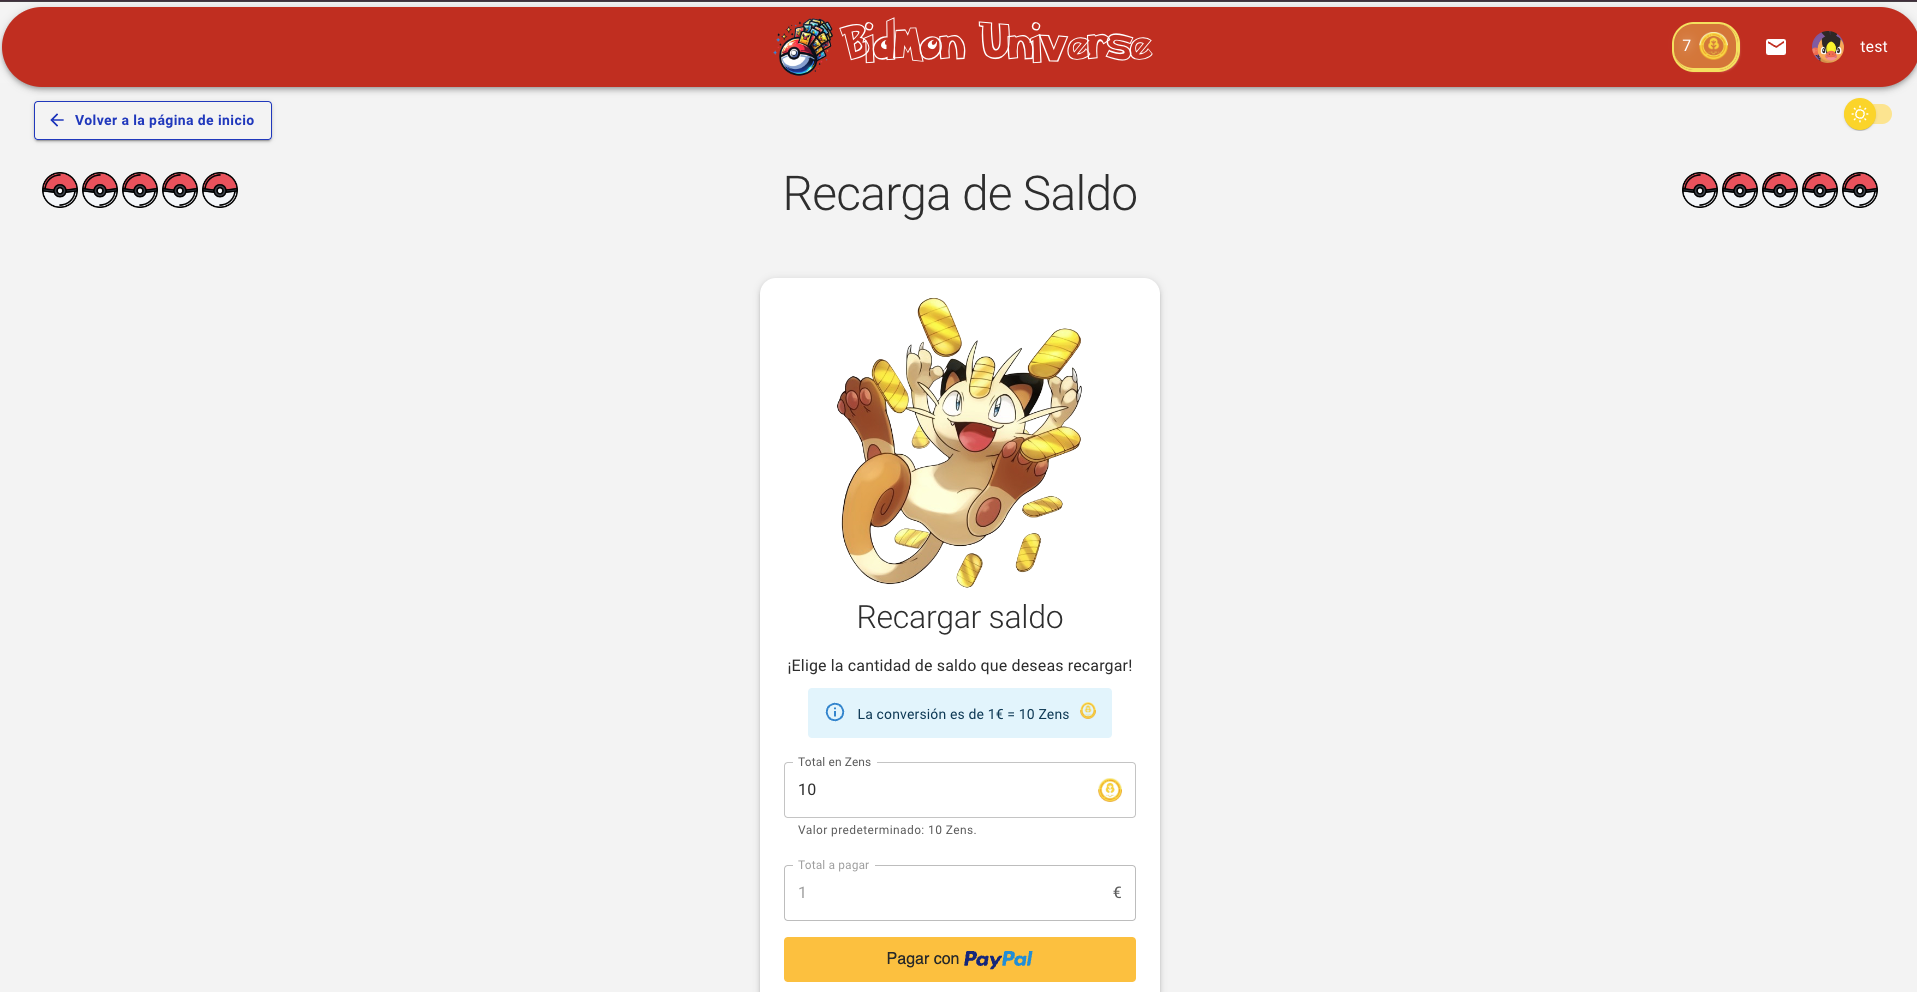
\includegraphics[width=0.8\textwidth]{figures/6-Analisis/6-Interfaz/interfaz/recarga.png}
    \caption{Página de recarga de saldo de la aplicación.}
    \label{fig:interfaz-recarga}
\end{figure}


\begin{figure}[H]
    \centering
    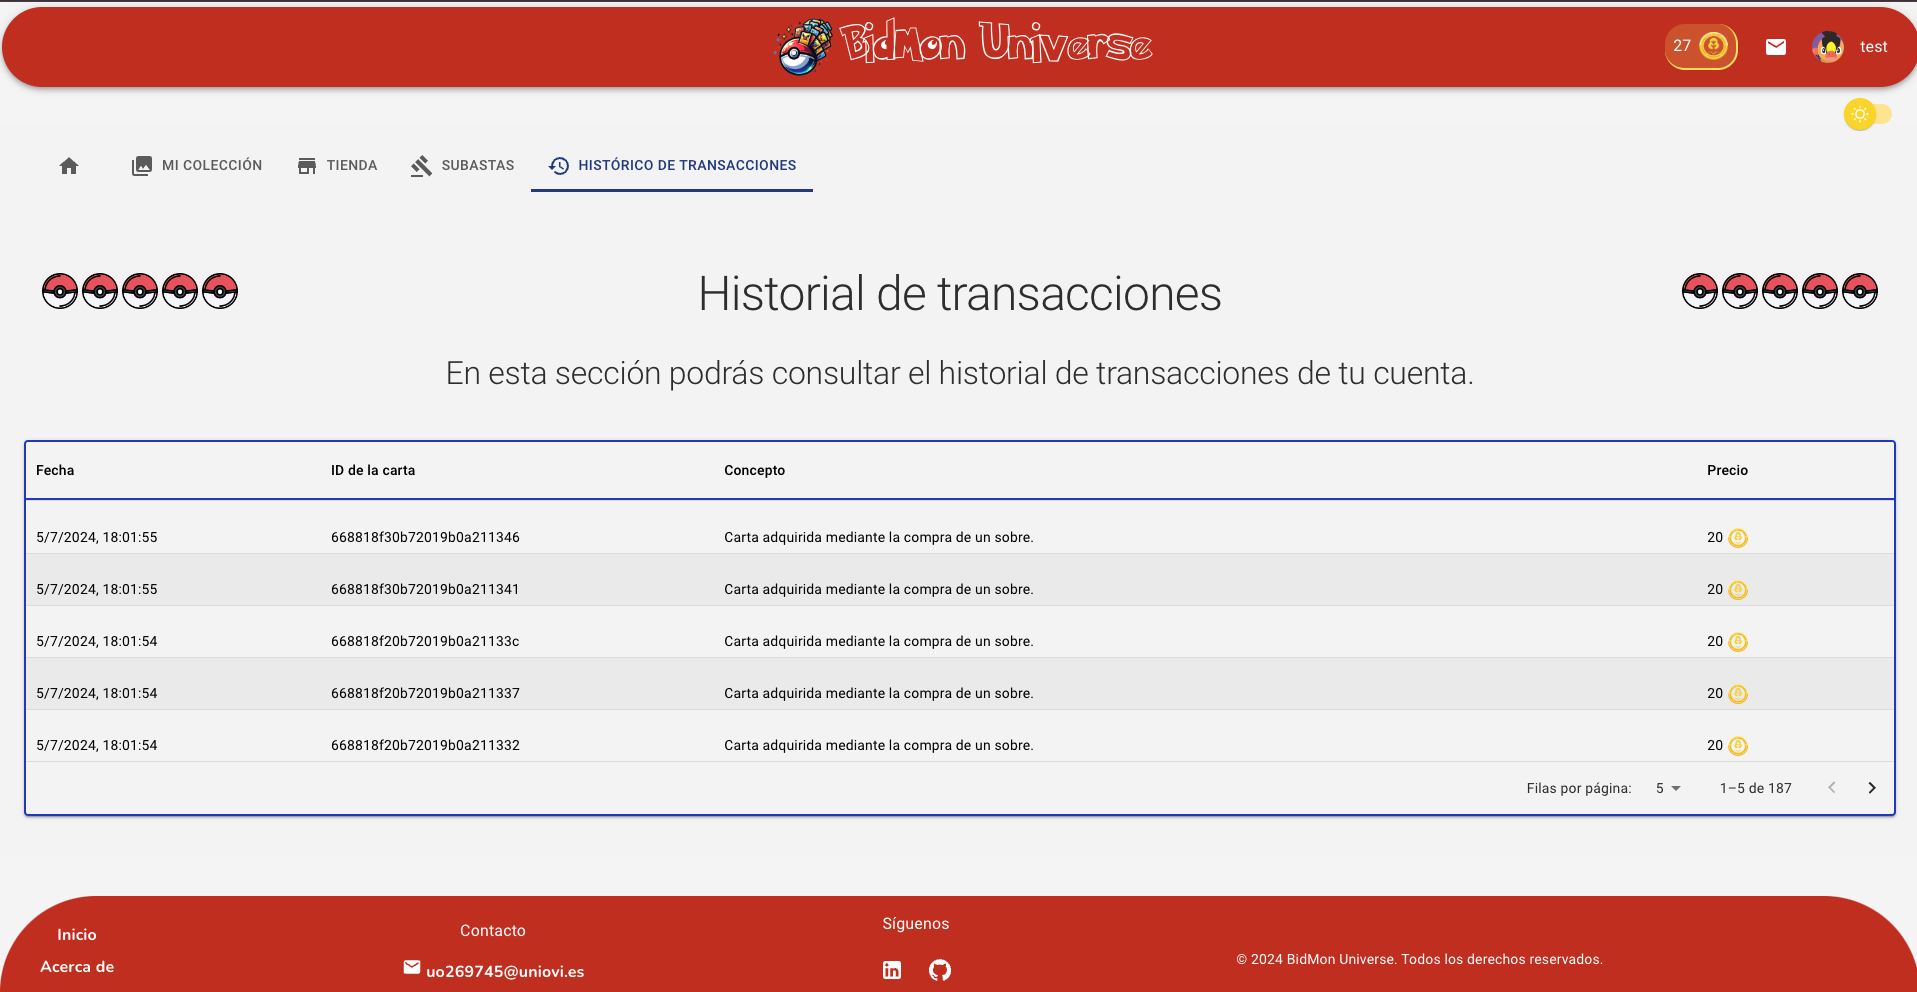
\includegraphics[width=0.8\textwidth]{figures/6-Analisis/6-Interfaz/interfaz/transacciones.png}
    \caption{Página de transacciones realizadas por el usuario.}
    \label{fig:interfaz-transacciones}
\end{figure}

\begin{figure}[H]
    \centering
    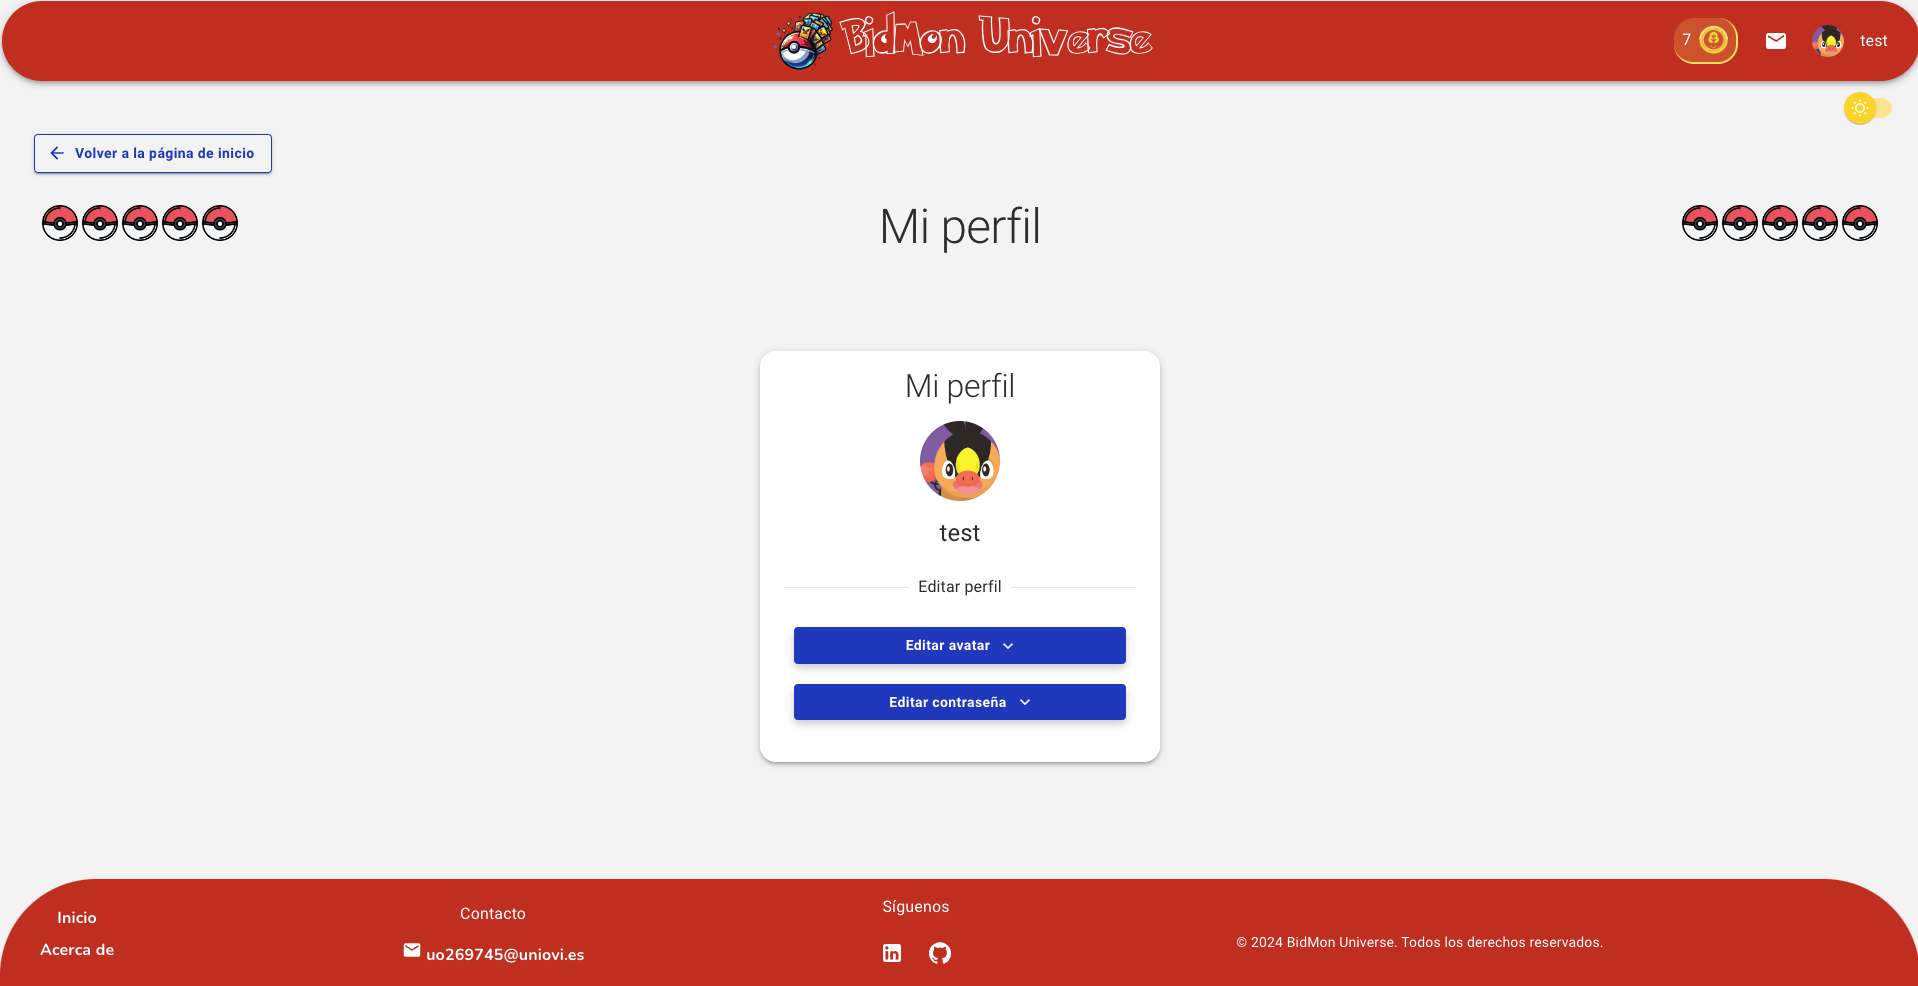
\includegraphics[width=0.8\textwidth]{figures/6-Analisis/6-Interfaz/interfaz/perfil1.png}
    \caption{Página de perfil del usuario.}
    \label{fig:interfaz-perfil1}
\end{figure}


\begin{figure}[H]
    \centering
    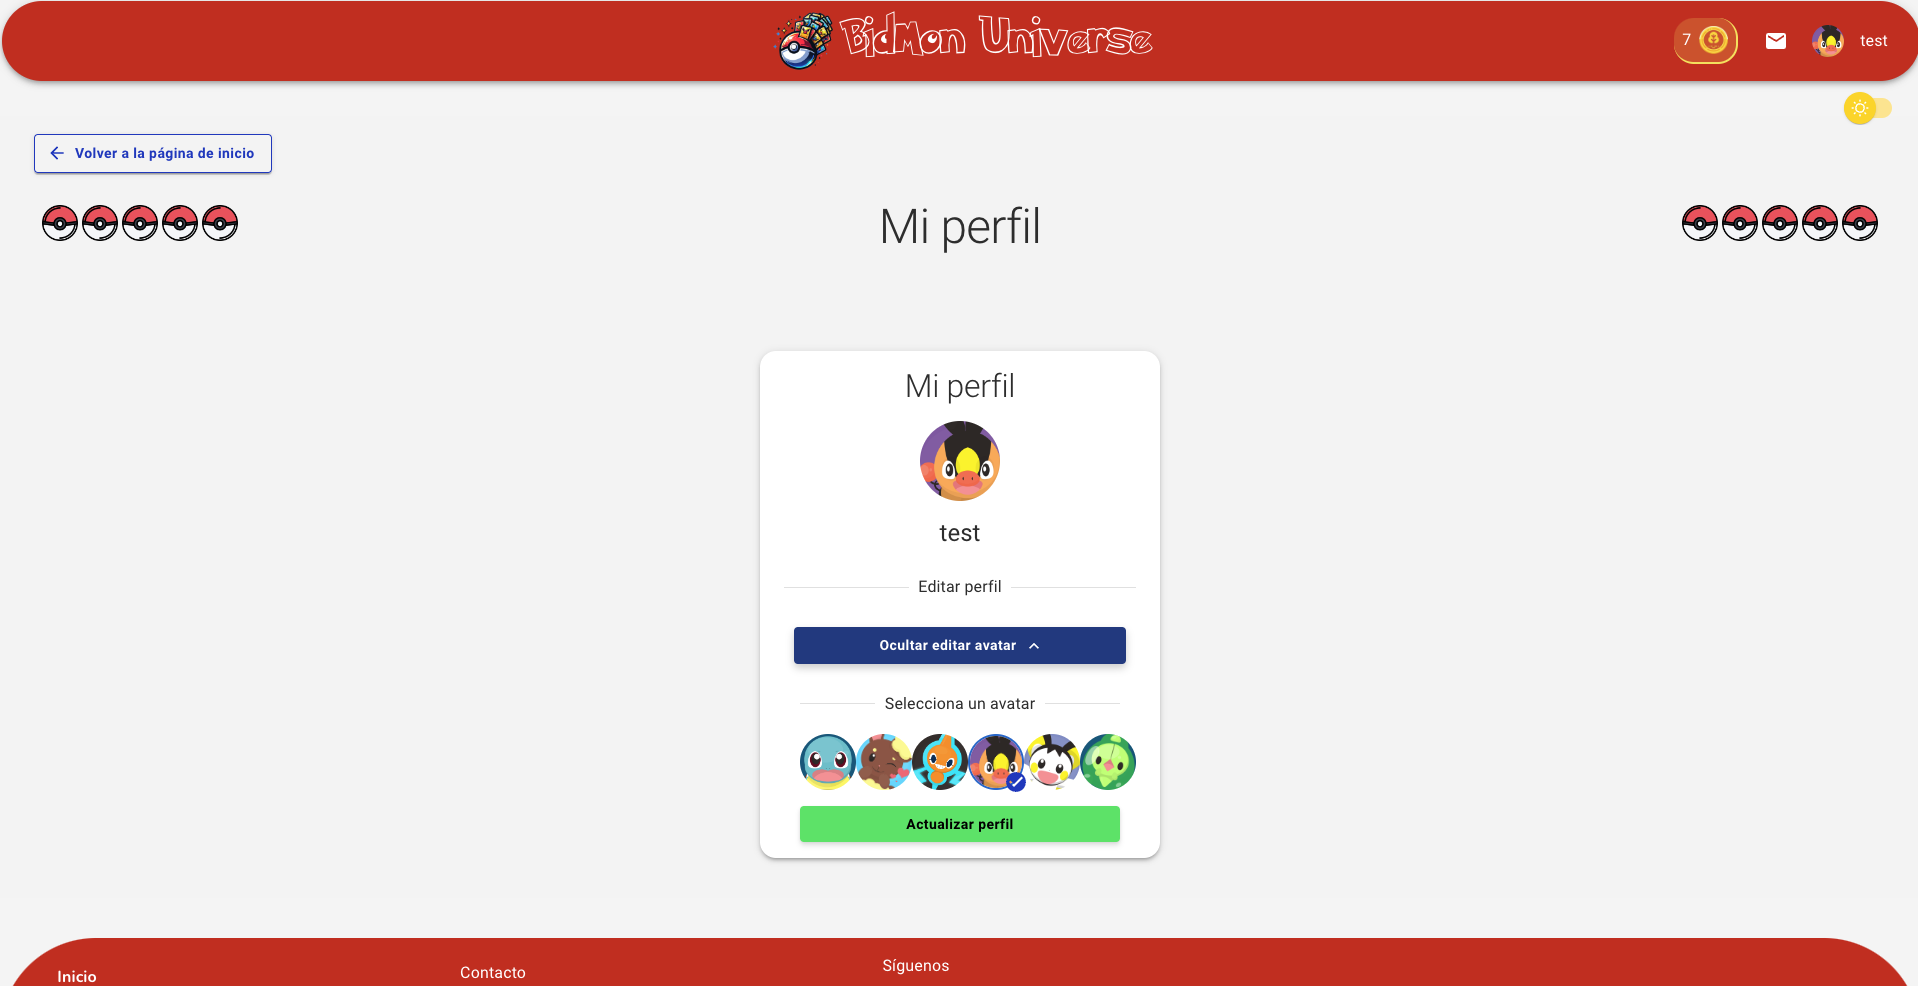
\includegraphics[width=0.8\textwidth]{figures/6-Analisis/6-Interfaz/interfaz/perfil2.png}
    \caption{Página de perfil del usuario, con la opción de cambiar la imagen de perfil desplegada.}
    \label{fig:interfaz-perfil2}
\end{figure}


\begin{figure}[H]
    \centering
    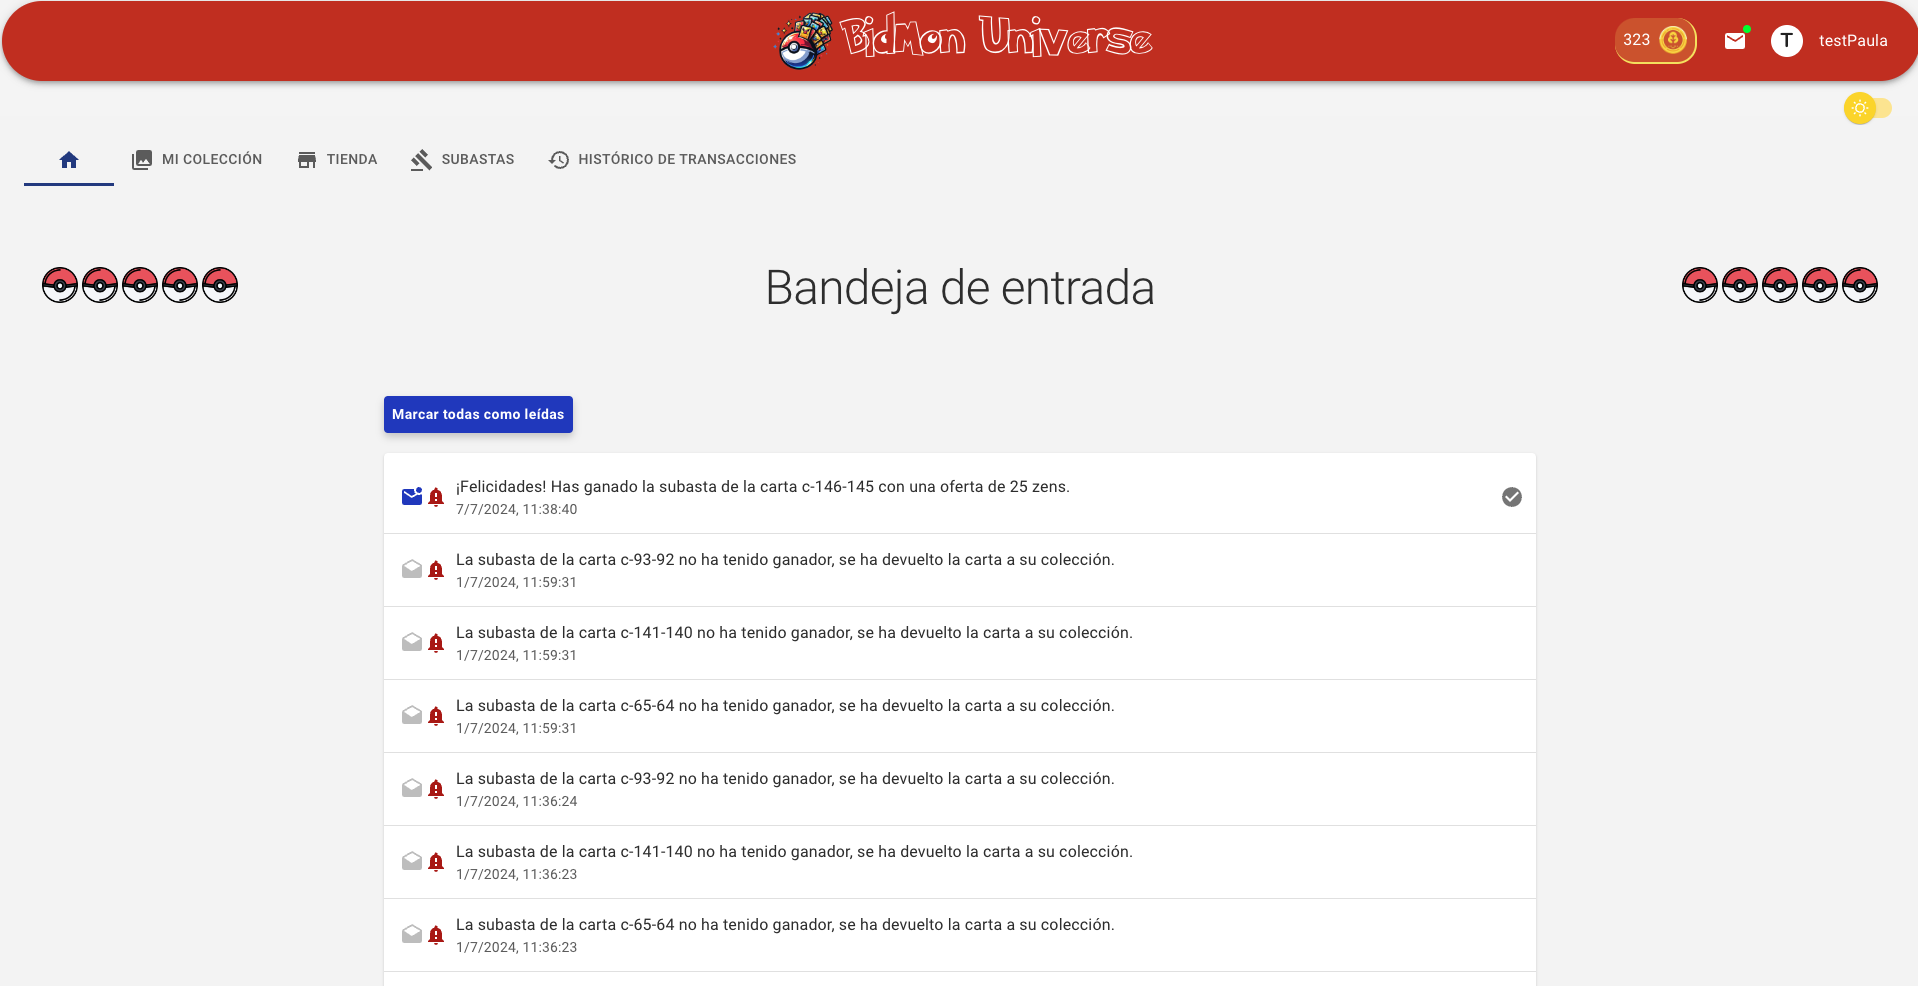
\includegraphics[width=0.8\textwidth]{figures/6-Analisis/6-Interfaz/interfaz/notificaciones_2.png}
    \caption{Página de notificaciones del usuario.}
    \label{fig:interfaz-notificaciones}
\end{figure}


El usuario puede elegir entre dos temas de la aplicación: el tema claro y el tema oscuro.
El tema claro es el que se muestra en las imágenes anteriores.
A continuación se adjuntan un par de imágenes de la aplicación en el tema oscuro, la página de inicio
y la página de pujas activas del usuario.

\begin{figure}[H]
    \centering
    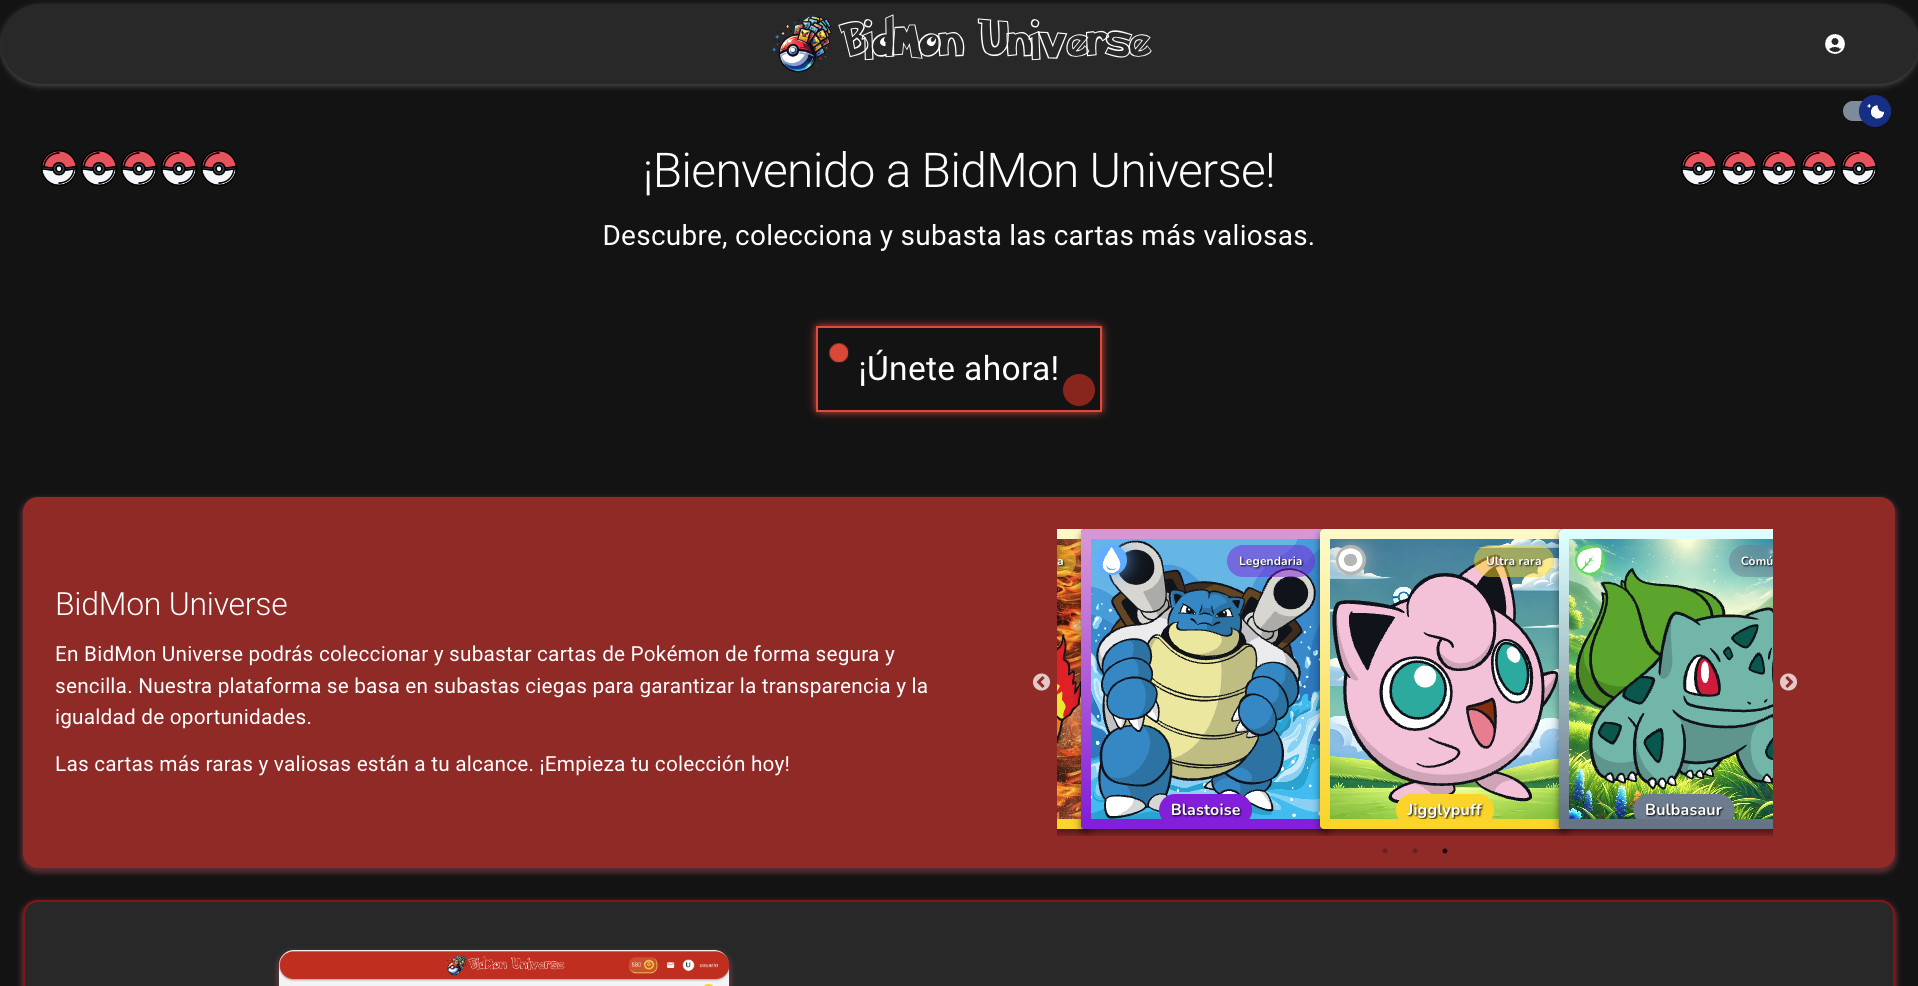
\includegraphics[width=0.8\textwidth]{figures/6-Analisis/6-Interfaz/interfaz/home_dark.png}
    \caption{Página Home en tema oscuro.}
    \label{fig:interfaz-home-dark}
\end{figure}

\begin{figure}[H]
    \centering
    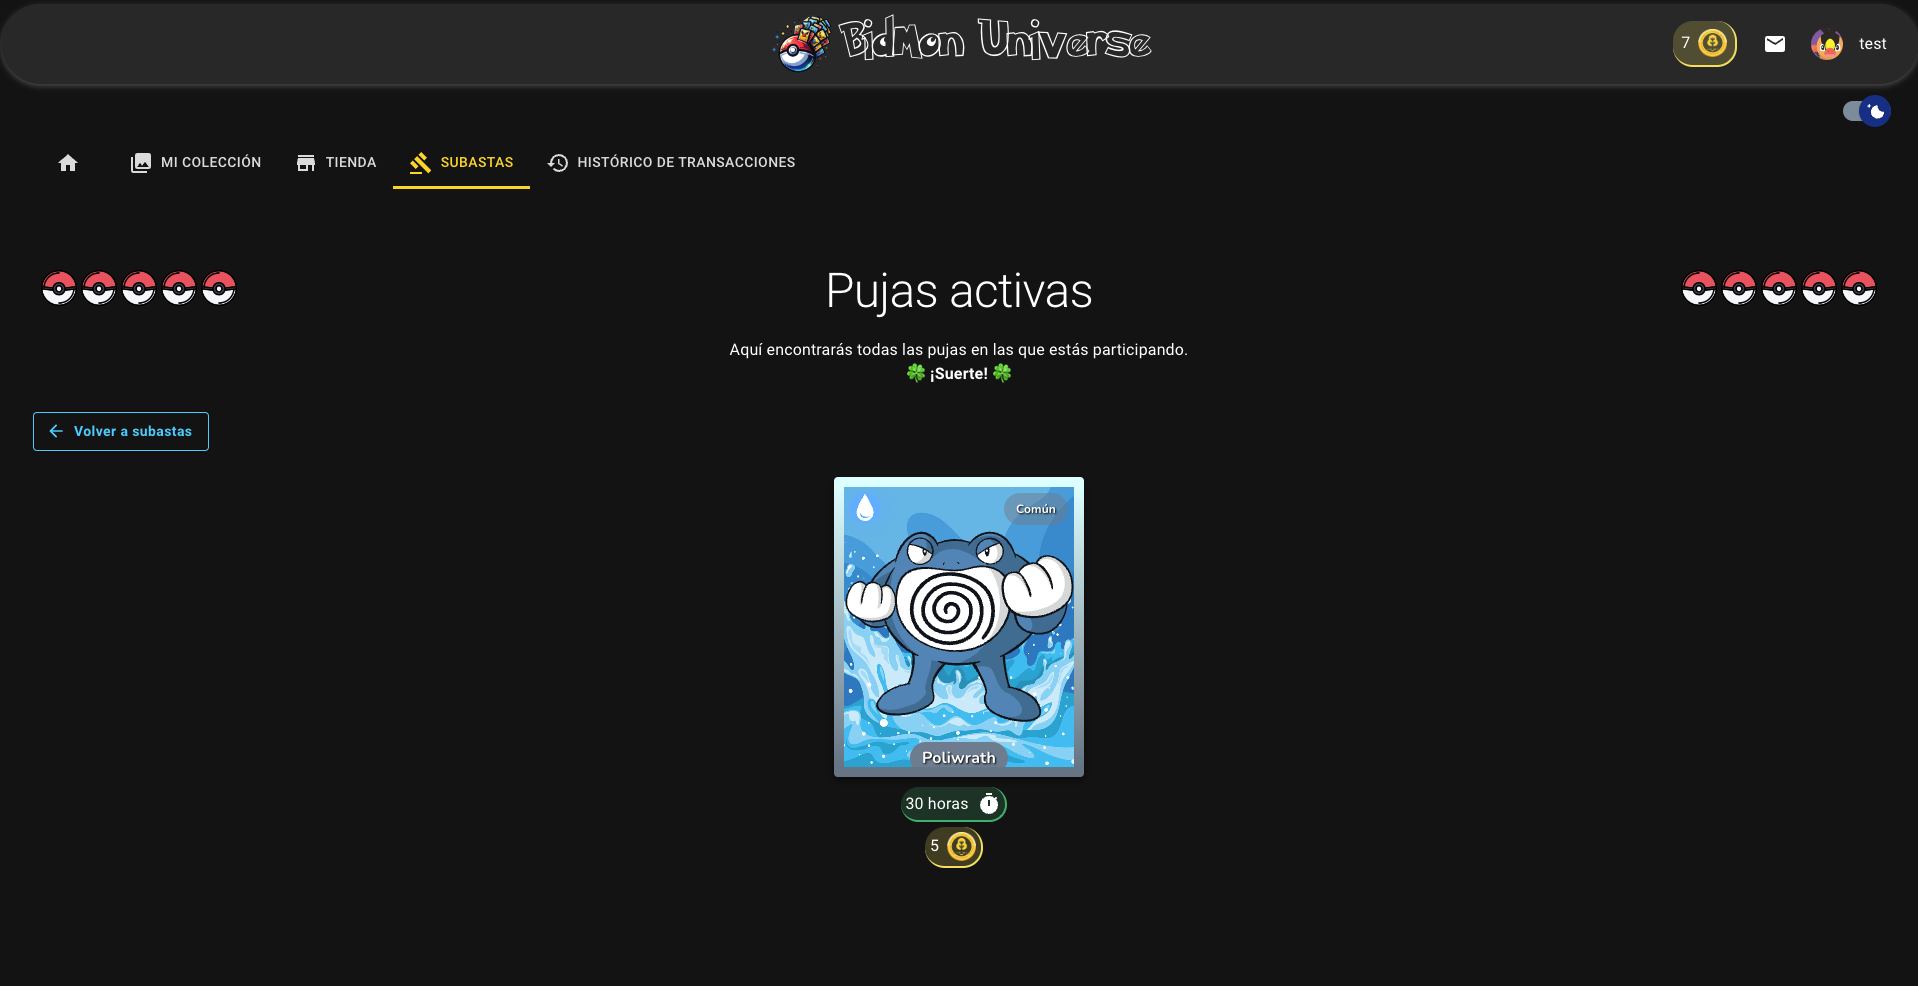
\includegraphics[width=0.8\textwidth]{figures/6-Analisis/6-Interfaz/interfaz/pujas_dark.png}
    \caption{Página de pujas activas del usuario en tema oscuro.}
    \label{fig:interfaz-pujas-dark}
\end{figure}